%%%%%%%%%%%%%%%%%%%%%%%%%%%%%%%%%%%%%%%%%%%%%%%%%%%%%%%%%%%%%%%%%%%%%%%%%%%%%%%%
%
% Template license:
% CC BY-NC-SA 3.0 (http://creativecommons.org/licenses/by-nc-sa/3.0/)
%
%%%%%%%%%%%%%%%%%%%%%%%%%%%%%%%%%%%%%%%%%%%%%%%%%%%%%%%%%%%%%%%%%%%%%%%%%%%%%%%%

%----------------------------------------------------------------------------------------
%	PACKAGES AND OTHER DOCUMENT CONFIGURATIONS
%----------------------------------------------------------------------------------------

\documentclass[
11pt, % The default document font size, options: 10pt, 11pt, 12pt
%oneside, % Two side (alternating margins) for binding by default, uncomment to switch to one side
%chapterinoneline,% Have the chapter title next to the number in one single line
spanish,
singlespacing, % Single line spacing, alternatives: onehalfspacing or doublespacing
%draft, % Uncomment to enable draft mode (no pictures, no links, overfull hboxes indicated)
%nolistspacing, % If the document is onehalfspacing or doublespacing, uncomment this to set spacing in lists to single
%liststotoc, % Uncomment to add the list of figures/tables/etc to the table of contents
%toctotoc, % Uncomment to add the main table of contents to the table of contents
parskip, % Uncomment to add space between paragraphs
%codirector, % Uncomment to add a codirector to the title page
headsepline, % Uncomment to get a line under the header
]{MastersDoctoralThesis} % The class file specifying the document structure



%----------------------------------------------------------------------------------------
%	INFORMACIÓN DE LA MEMORIA
%----------------------------------------------------------------------------------------

\thesistitle{Prototipo de dispositivo de geolocalización basado en tecnología GNSS} % El títulos de la memoria, se usa en la carátula y se puede usar el cualquier lugar del documento con el comando \ttitle

% Nombre del posgrado, se usa en la carátula y se puede usar el cualquier lugar del documento con el comando \degreename
\posgrado{Carrera de Especialización en Sistemas Embebidos} 
%\posgrado{Carrera de Especialización en Internet de las Cosas} 
%\posgrado{Carrera de Especialización en Intelegencia Artificial}
%\posgrado{Maestría en Sistemas Embebidos} 
%\posgrado{Maestría en Internet de las cosas}

\author{Ing. Luis David Díaz Charris} % Tu nombre, se usa en la carátula y se puede usar el cualquier lugar del documento con el comando \authorname

\director{Esp. Ing. Santiago Esteva (FIUBA)} % El nombre del director, se usa en la carátula y se puede usar el cualquier lugar del documento con el comando \dirname
\codirector{Nombre del codirector (pertenencia)} % El nombre del codirector si lo hubiera, se usa en la carátula y se puede usar el cualquier lugar del documento con el comando \codirname.  Para activar este campo se debe descomentar la opción "codirector" en el comando \documentclass, línea 23.

\juradoUNO{Dr. Ing. Javier Jiménez (Universidad de la Costa, CUC)} % Nombre y pertenencia del un jurado se usa en la carátula y se puede usar el cualquier lugar del documento con el comando \jur1name
\juradoDOS{Dr. Ing. Emiro De La Hoz (Universidad de la Costa, CUC)} % Nombre y pertenencia del un jurado se usa en la carátula y se puede usar el cualquier lugar del documento con el comando \jur2name
\juradoTRES{Mg. Ing. Jorge Díaz (Universidad de la Costa, CUC)} % Nombre y pertenencia del un jurado se usa en la carátula y se puede usar el cualquier lugar del documento con el comando \jur3name

%\ciudad{Ciudad Autónoma de Buenos Aires}
\ciudad{ciudad de Barranquilla, Colombia}

\fechaINICIO{marzo de 2023}
\fechaFINAL{agosto de 2024}


\keywords{Sistemas embebidos, GNSS, Geolocalización, FIUBA} % Keywords for your thesis, print it elsewhere with \keywordnames
\usepackage{geometry}
\usepackage{array}
\usepackage{comment}
\usepackage{hyperref}
\usepackage{pdfpages}
\usepackage{pdflscape}


%\usepackage[]{biblatex}
%\addbibresource{references.bib}

%%\begin{comment}
\maxdeadcycles=200


\lstset{
  language=C,             % Define el lenguaje del código (puedes cambiarlo a tu necesidad)
  basicstyle=\color{black}\ttfamily\small,  % Define el estilo básico del texto del código
  keywordstyle=\color{blue},   % Define el estilo para las palabras clave
  commentstyle=\color{green},  % Define el estilo para los comentarios
  stringstyle=\color{red},     % Define el estilo para las cadenas de texto
  numbers=left,                % Coloca los números de línea a la izquierda
  numberstyle=\tiny\color{gray}, % Estilo de los números de línea
  stepnumber=1,                % Numera cada línea
  numbersep=10pt,              % Espacio entre los números de línea y el código
  backgroundcolor=\color{white}, % Fondo blanco para el código
  frame=single,                % Marco alrededor del código
  breaklines=true,             % Permite romper líneas largas
  breakatwhitespace=false,     % Rompe líneas en cualquier espacio en blanco
  postbreak=\mbox{\textcolor{red}{$\hookrightarrow$}\space} % Caracter para indicar líneas continuadas
}
%%\end{comment}


\begin{document}


\frontmatter % Use roman page numbering style (i, ii, iii, iv...) for the pre-content pages

\pagestyle{plain} % Default to the plain heading style until the thesis style is called for the body content


%----------------------------------------------------------------------------------------
%	RESUMEN - ABSTRACT 
%----------------------------------------------------------------------------------------

\begin{abstract}
\addchaptertocentry{\abstractname} % Add the abstract to the table of contents
%
%The Thesis Abstract is written here (and usually kept to just this page). The page is kept centered vertically so can expand into the blank space above the title too\ldots
\centering

En esta memoria se describe el diseño y desarrollo de un prototipo de dispositivo de geolocalización basado en tecnología GNSS. Este permite reportar la posición geográfica de una cava móvil de transporte de alimentos con una precisión mínima de diez metros. El prototipo implementa un receptor de señales GNSS capaz de recibir simultáneamente señales de los sistemas GPS y BeiDou. Además de incorporar comunicación 4G, lo que permite la posibilidad de transmitir datos vía internet a una aplicación web de monitoreo en tiempo real. 

Para el desarrollo del presente trabajo, se aplicaron todos los conocimientos en planificación y gestión de proyectos, ingeniería del software para sistemas embebidos, programación de microcontroladores, sistemas operativos en tiempo real, diseño de circuitos impresos y protocolos de comunicación. 

\end{abstract}

%----------------------------------------------------------------------------------------
%	CONTENIDO DE LA MEMORIA  - AGRADECIMIENTOS
%----------------------------------------------------------------------------------------

\begin{acknowledgements}
%\addchaptertocentry{\acknowledgementname} % Descomentando esta línea se puede agregar los agradecimientos al índice
\vspace{1.5cm}

Agradezco a Dios por su infinita misericordia. 

Agradezco a mi esposa Yuranys, por su aguante para conmigo. 

Agradezco enormemente a Ariel Lutenberg por la oportunidad, la confianza y sus inacabables ganas de ayudar. 

Agradezco a Martín Menéndez, a Santiago Germino y a Ramiro Ghignone por darme un lugar en su grupo. 

Agradezco a Santiago Esteva por su guía en este trabajo. 

\end{acknowledgements}

%----------------------------------------------------------------------------------------
%	LISTA DE CONTENIDOS/FIGURAS/TABLAS
%----------------------------------------------------------------------------------------

\tableofcontents % Prints the main table of contents

\listoffigures % Prints the list of figures

\listoftables % Prints the list of tables


%----------------------------------------------------------------------------------------
%	CONTENIDO DE LA MEMORIA  - DEDICATORIA
%----------------------------------------------------------------------------------------

\dedicatory{\textbf{Dedicado a...}

Mis hijos, Tomás y María Helena, son lo mejor de mi vida. 

Mi esposa Yuranys.

Mi madre Luz Fabiola. 
}  % escribir acá si se desea una dedicatoria


%----------------------------------------------------------------------------------------
%	CONTENIDO DE LA MEMORIA  - CAPÍTULOS
%----------------------------------------------------------------------------------------

\mainmatter % Begin numeric (1,2,3...) page numbering

\pagestyle{thesis} % Return the page headers back to the "thesis" style

% Incluir los capítulos como archivos separados desde la carpeta Chapters

% Chapter 1

\chapter{Introducción general} % Main chapter title

\label{Chapter1} % For referencing the chapter elsewhere, use \ref{Chapter1} 
\label{IntroGeneral}

En este capítulo se exponen los aspectos fundamentales del trabajo, con el propósito de familiarizar al lector con las estrategias de desarrollo que se detallan en los capítulos subsiguientes.

%----------------------------------------------------------------------------------------

% Define some commands to keep the formatting separated from the content 
\newcommand{\keyword}[1]{\textbf{#1}}
\newcommand{\tabhead}[1]{\textbf{#1}}
\newcommand{\code}[1]{\texttt{#1}}
\newcommand{\file}[1]{\texttt{\bfseries#1}}
\newcommand{\option}[1]{\texttt{\itshape#1}}
\newcommand{\grados}{$^{\circ}$}

%----------------------------------------------------------------------------------------

%\section{Introducción}

%----------------------------------------------------------------------------------------

\section{Descripción del proyecto}
\label{sec:desc_general}

A continuación, se presenta una descripción del contexto, problema y propuesta de solución que guiaron el presente trabajo.

\subsection{Contexto y problema}

Una cadena de supermercados en Colombia tiene importantes retos logísticos a la hora de abastecer las tiendas distribuidas en todas las ciudades. La empresa implementa centros de abastecimiento que cubren distintas ciudades en determinados rangos de acción. Uno de los retos más relevantes a los que se enfrenta, es la distribución de alimentos en cadena de frío. Dicha tarea, se lleva a cabo a través de cavas móviles que tienen la capacidad de conservar la temperatura interna y refrigerar su interior. Estas cavas representan un activo costoso y son totalmente reutilizables. En la figura \ref{fig:cava}, se puede apreciar un ejemplo de cava móvil para transporte de alimentos. 

\vspace{1cm}

\begin{figure}[htbp]
	\centering
	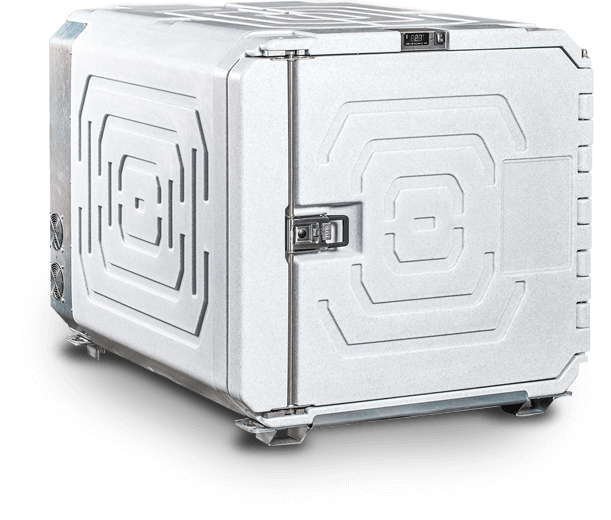
\includegraphics[width=.5\textwidth]{./Figures/cava.png}
	\caption{Ejemplo de una cava móvil\protect\footnotemark.}
	\label{fig:cava}
\end{figure}
\footnotetext{\url{https://www.coldtainer.es}}

El centro de despacho enfrenta problemas logísticos cuando se queda sin cavas disponibles para la distribución. En esta situación, es necesario realizar un esfuerzo adicional para ubicar y recuperar las cavas. La dificultad radica en que no es posible saber su ubicación exacta en tiempo real. Por lo tanto, se requiere solicitar a cada sucursal el reporte de cavas disponibles para su retorno al centro de distribución.

\subsection{Alternativa de solución}

Por lo anterior, se planteó como una alternativa de solución, el desarrollo de un dispositivo que permita rastrear la ubicación de cada una de las cavas. Este dispositivo permite replicarse con facilidad, es de bajo consumo de energía y tiene una precisión de diez metros en el reporte de ubicación de las cavas. 


%----------------------------------------------------------------------------------------

\section{Estado del arte}
\label{sec:estado_del_arte}

Los sistemas de navegación por satélite son actualmente las herramientas por excelencia en las aplicaciones de movilidad y transporte. El geo-posicionamiento es una utilidad necesaria en todos los tipos de transporte: navegación espacial, la aviación, la navegación marítima, los ferrocarriles y el transporte automotor por carretera \citep{GNSS-Junta-Adalucia}.

Uno de los sistemas de navegación más conocidos es el Sistema de Posicionamiento Global (GPS), desarrollado por el Departamento de Defensa de Estados Unidos. Sin embargo, a nivel mundial existen varios de estos sistemas, y al conjunto de ellos se le conoce como Sistemas de Navegación Global por Satélite (GNSS, del inglés Global Navigation Satellite Systems) \citep{GNSS-ONU}. Los GNSS están compuestos por constelaciones de satélites que orbitan la Tierra y transmiten datos sobre su ubicación espacial y temporal. Además, incluyen redes de estaciones de control terrestres y receptores que calculan las posiciones en tierra mediante la técnica de trilateración \citep{GNSS-ONU}. 

Algunos de los GNSS que existen actualmente son \citep{GNSS-Junta-Adalucia}:

\begin{itemize}
    \item El Sistema GPS (Global Position System): de EE. UU., con 30 satélites, a una altura de 20 200 km.
    \item El Sistema Glonass (Global Orbiting Navigation Satellite System): de Rusia, con 24 satélites, a una altura de 25 500 km.
    \item El Sistema Galileo (ESA): de Europa, con 30 satélites, a una altura de 23 200 km.
    \item El Sistema BeiDou (BDS): de China, con 34 satélites, a una altura entre 21 600 km. y 35 800  km.
\end{itemize}

En la literatura científica, estos sistemas son ampliamente estudiados y revisados, debido a su gran rango de aplicaciones en diferentes áreas del conocimiento (aparte de la navegación) y la técnica. Entre las más relevantes se destacan:

\begin{itemize}
    \item Ingeniería Civil y Arquitectura. Por ejemplo, para el replanteo de infraestructuras y estructuras, control del movimiento de tierras, medición de perfiles transversales, entre otras.
    \item Cartografía y Topografía, para mejorar la precisión de la cartografía y la modelización del mundo físico, desde montañas y ríos, hasta calles, edificios, cables y tuberías de los servicios públicos.
    \item Geodesia y Geofísica, para mejorar la precisión en el estudio de los fenómenos físicos que afectan la forma y dimensiones de la Tierra.
    \item Agricultura en el desarrollo de mejores técnicas para la gestión de los cultivos. 
\end{itemize}

\subsection{Antecedentes}

A continuación, se presentan algunos antecedentes en la literatura científica sobre el estudio de los sistemas GNSS. 

\textit{Di Garzia et al.} \citep{DiGrazia} evaluaron el rendimiento del chip receptor de GNSS TeseoV STA8135GA, de STMicroelectronics. Su trabajo se contextualiza en las aplicaciones automotrices de alta precisión. Determinaron la viabilidad técnica y las ventajas de que en un solo chip se pudiera incorporar la capacidad de recibir señales de tres bandas. Lo anterior, permitió agregar resiliencia y redundancia en caso de fallas completas de alguna de las bandas de frecuencia. 

\textit{Shu et al.}  \citep{Shu} evaluaron el rendimiento de un GNSS multi-constelación para averiguar el impacto en la determinación de la posición en un ambiente dinámico. Lo anterior, para saber cuánto mejora el GNSS la precisión de la posición. Con su estudio determinaron que:

\begin{itemize}
    \item En un caso estático, los sistemas GPS, GLONASS y BeiDou tienen el mismo rendimiento.
    \item En el caso dinámico, los sistemas GPS y GLONASS tienen rendimientos muy similares, donde el de GPS es superior. 
    \item Cuando se combinan GPS, BeiDou, GLONASS y Galileo, la respuesta es significativamente mejor en comparación con el empleo de un único sistema de posicionamiento. 
\end{itemize}

Por su parte, \textit{Villien y Denis} \citep{Villien} emplean una combinación de tres estrategias para mejorar la calidad de la recepción GNSS:

\begin{enumerate}
    \item Utilizan un receptor GNSS de múltiples constelaciones y para ampliar el rango de transmisores satelitales de los que obtener información de posicionamiento. 
    \item Utilizan una antena de banda ultra ancha (UWB, del inglés ultra-wideband) para optimizar en una única antena la capacidad de recibir señales GNSS con un ancho de banda amplio.
    \item Emplean una unidad de medida inercial junto con un filtro Kalman. Esta configuración permite rastrear de forma completa el objeto observado y reducir la carga computacional del sistema.
\end{enumerate}

El trabajo de \textit{Villien y Denis} logra un posicionamiento con una precisión de alcance entre 3 cm y 11 cm en entornos controlados. Además, se evidencia una precisión horizontal en las mediciones GNSS superior a 40 cm durante una prueba de campo, incluso en condiciones degradadas de recepción de la señal GNSS. Este trabajo es especialmente relevante en aplicaciones de geo-posicionamiento en espacios cerrados o túneles, donde un único sistema GNSS resulta insuficiente. 




%----------------------------------------------------------------------------------------

\section{Objetivos y alcance}
\label{sec:objetivos}

\subsection{Objetivo general} 

Desarrollar un prototipo de dispositivo de geolocalización basado en tecnología GNSS, que permita reportar y hacer seguimiento en tiempo real de la posición geográfica de una cava móvil de transporte de alimentos con una precisión mínima de diez metros.


\subsection{Objetivos específicos} 

\begin{enumerate}
    \item Diseñar la arquitectura de hardware y firmware, del dispositivo de geolocalización con tecnología GNSS. 
    \item Implementar el hardware y el firmware del dispositivo de geolocalización.
    \item Implementar un servicio online para el seguimiento de la posición geográfica.
    \item Realizar pruebas de consumo energético, precisión y funcionalidad del prototipo.
\end{enumerate}


\subsection{Alcance} 

Este trabajo abordó:
\begin{itemize}
    \item El análisis de métodos ingenieriles adecuados y tecnologías disponibles para la implementación del sistema.
    \item El diseño y prototipado del sistema y subsistemas de hardware requerido para la interconexión con los sistemas GNSS y la red celular. 
    \item El diseño y prototipado del sistema y subsistemas de hardware requerido para la interfaz humano-máquina tales como pilotos, teclas o pantallas. 
    \item El desarrollo del firmware necesario para ejecutar las funciones de conectividad, funciones lógicas y reporte de estados.
    \item Configuración de la API web necesaria para realizar pruebas de seguimiento en tiempo real del dispositivo. 
    \item Optimización del consumo de energía a través de firmware.
\end{itemize}

Este trabajo no incluyó:

\begin{itemize}
    \item El desarrollo de una interfaz web a medida.
    \item El diseño del aspecto físico del dispositivo. 
\end{itemize}



%----------------------------------------------------------------------------------------
\chapter{Introducción específica} % Main chapter title

\label{Chapter2}

%----------------------------------------------------------------------------------------

Este capítulo presenta en detalle los temas aplicados en el desarrollo del trabajo y las definiciones realizadas en el inicio del trabajo. Permite conocer los requisitos y organización de tareas planteados.



%----------------------------------------------------------------------------------------

\section{Requerimientos}
\label{sec:requerimientos}

A continuación,  se presentan los requerimientos planteados en la planificación del trabajo:

\begin{enumerate}
	\item Requerimientos funcionales
		\begin{enumerate}
            \item El sistema a desarrollar debe ser un prototipo funcional para pruebas en ambiente de laboratorio. 
			\item El sistema debe reportar en una plataforma de software la posición geográfica de las cavas en tiempo real.
            \item La plataforma de software deberá permitir la visualización en un mapa de la posición geográfica de las cavas.
			\item La precisión del reporte de la posición geográfica debe ser de diez metros (10 m). 
            \item Como requisito mínimo, el sistema debe ser capaz de conectarse con dos constelaciones de satélites para obtener la posición geográfica.  
            \item El hardware debe tener botones para que los operarios puedan reportar la ocupación o desocupación de las cavas. 
            \item El hardware debe poseer un display LCD que permita a los operarios visualizar las coordenadas geográficas reportadas por el sistema y el estado de ocupación de la cava. 
            \item El hardware debe poseer pilotos que permitan a los usuarios visualizar e interpretar de forma lógica el estado de ocupación de las cavas. 
		\end{enumerate}
	\item Requerimientos no funcionales
		\begin{enumerate}
			\item El sistema debe ser escalable y debe poderse replicar. 
			\item El sistema a desarrollar debe usar componentes electrónicos disponibles en Colombia. 
		\end{enumerate}
\end{enumerate}





%----------------------------------------------------------------------------------------

\section{Estructura del sistema}
\label{sec:Estructura_sistema}

En la figura ~\ref{fig:diagrama_general} se observa el diagrama general del prototipo que se construyó. Allí se representa al microcontrolador, que funge como unidad de procesamiento central. Además, se distinguen los componentes de comunicación satelital y celular: un receptor GNSS y un módulo 4G LTE. Se aprecian, las infraestructuras de comunicación que se emplearon para hacer posible la comunicación. Se distingue la infaltable fuente de alimentación para garantizar la energía. Por último, el sistema comprende de una interfaz web como herramienta para la presentación y seguimiento de la información. 

En el capítulo siguiente se aborda con más detalle la implementación de cada uno de estos módulos.


\vspace{1cm}

\begin{figure}[htbp]
	\centering
	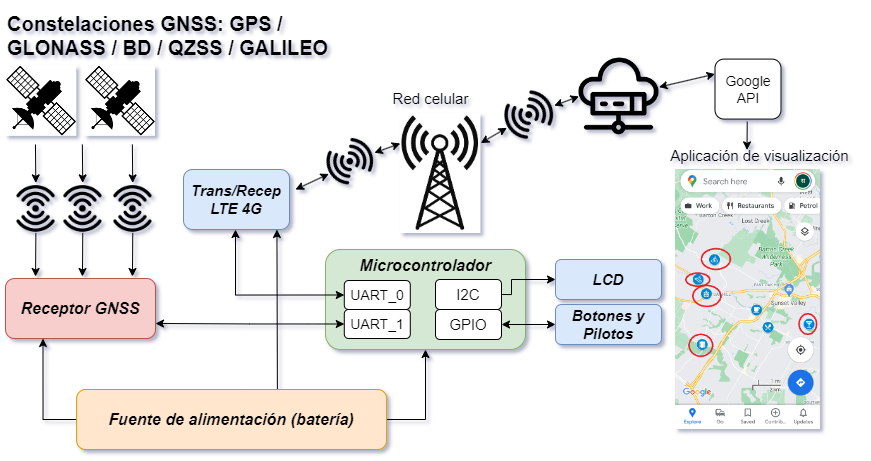
\includegraphics[width=1\textwidth]{./Figures/diagrama_general.png}
	\caption{Diagrama general del sistema.}
	\label{fig:diagrama_general}
\end{figure}


%----------------------------------------------------------------------------------------

\section{Componentes del sistema}
\label{sec:Componentes_sistema}

En este trabajo se desarrolló un prototipo para realizar el posicionamiento geográfico de cavas móviles de transporte de alimentos. Dicho sistema comprende los siguientes componentes:

\begin{itemize}
    \item Microcontrolador, que realiza las labores de unidad central de procesamiento.
    \item Receptor GNSS, para la recepción de datos de posicionamiento.
    \item Módulo de comunicación 4G, para la conexión a Internet.
    \item Plataforma de software para la presentación de la información. 
    \item Fuente de alimentación.
\end{itemize}

Para la selección de los principales componentes se buscaron alternativas en el mercado a partir de los requisitos planteados en la sección ~\ref{sec:requerimientos}.

\subsection{Microcontrolador ESP32}
\label{Microcontrolador}

Luego de realizar un estudio comparativo entre tres plataformas de microcontroladores disponibles en el mercado colombiano, se seleccionó el microcontrolador ESP32. En la tabla ~\ref{tabla:comparativa} se presenta un extracto de la comparación entre las plataformas. 

\begin{table}[h]
    \centering
    \caption{Tabla comparativa de Microcontroladores.}
    \begin{tabular}{p{3cm} p{3cm} p{2.5cm} p{2.5cm} }
    \toprule

        \textbf{Característica}           & \textbf{ESP-WRoom-32}               & \textbf{Arduino MEGA}               & \textbf{STM32 F401} \\
        \midrule
        \textbf{CPU}                    & Dual-core Tensilica Xtensa LX6     & ATmega2560 (8-bit)                  & ARM Cortex-M4 @ 84 MHz               \\
        
        \textbf{Número de núcleos}       & 2                                  & 1                                  & 1                                   \\
        
        \textbf{Frecuencia del procesador (MHz)}  & 160                       & 16                                 & 84                                  \\

        \textbf{ROM}             & 448 kB                             & 256 kB (Flash)                     & 512 kB (Flash)                      \\

        \textbf{RAM}             & 520 kB                             & 8 kB (SRAM)                        & 96 kB (SRAM)                        \\

        \textbf{Comunicación} & Wi-Fi, Bluetooth, 2x UART, 1x SPI, 1x I2C y 1x USB.    & 1x USB, 2x UART, 1x SPI e 1x I2C                 & 3x USART, 4x SPI, 3x I2C, 1x CAN y 1x USB  \\

        \textbf{Lenguajes de programación} & Arduino, C/C++ y Micropython  & Arduino y C/C++               & Arduino y C/C++                  \\

        \textbf{Cantidad de GPIO's }       & 36            & 54 (Digital), 16 (Analog)           & 82                                  \\

        \textbf{Soporte de hardware para RTOS} & Sí        & No 16 (Analog)           & Sí                                 \\
    \bottomrule
    \hline
    \end{tabular}
    \label{tabla:comparativa}
\end{table}


El microcontrolador ESP32 comprende una familia o serie de microcontroladores tipo System on Chip (SoC), desarrollado por la empresa Espressif \citep{ESPRESSIF}. 

El ESP32 es un sistema de doble núcleo con dos CPU Harvard Architecture Xtensa LX6. Toda la memoria integrada, la memoria externa y los periféricos se encuentran en el bus de datos y/o el bus de instrucciones de estas CPU. Las dos CPU se denominan PRO\_CPU y APP\_CPU (de protocolo y aplicación), sin embargo, para la mayoría de los propósitos las dos CPU son intercambiables \citep{ESPRESSIF}.

Entre las principales características de este microcontrolador se encuentran:

\begin{itemize}
    \item Espacio de direcciones de 4 GB (32 bits) para el bus de datos y el bus de instrucciones. 
    \item Espacio de direcciones DMA de 328 kB. Trece de sus módulos son capaces de operar con DMA.
    \item Espacio de direcciones periférico de 512 kB.
    \item ROM interna de 448 kB.
    \item SRAM interna de 520 kB.
    \item Admite hasta 16 MB de Flash SPI o hasta 8 MB de SPI SRAM.    
\end{itemize}

En la figura ~\ref{fig:ESP32} se presenta la placa de desarrollo ESP32-Devkit-V4.

\vspace{1cm}

\begin{figure}[htbp]
	\centering
	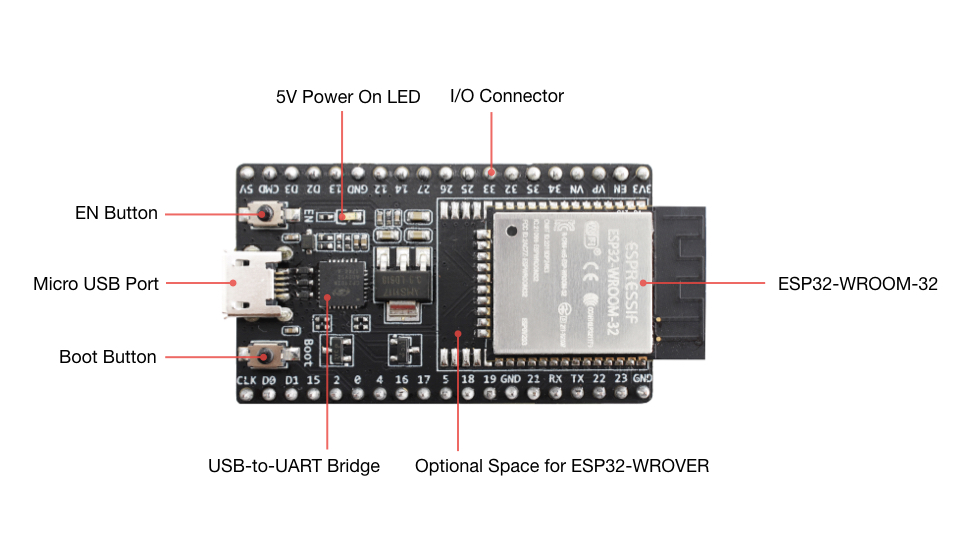
\includegraphics[width=1\textwidth]{./Figures/ESP32.jpg}
	\caption{Placa de desarrollo ESP32-Devkit-V1\protect\footnotemark.}
        
	\label{fig:ESP32}
\end{figure}
\footnotetext{Imagen tomada de: \url{https://docs.espressif.com/projects/esp-idf/en/latest/esp32/hw-reference/esp32/get-started-devkitc.html}}

A continuación, se presentan los beneficios de haber aplicado el microcontrolador ESP32 en el presente trabajo:

\begin{itemize}
    \item Es de resaltar la significativa capacidad de cómputo inherente a su diseño, ya que cuenta con un procesador de doble núcleo. Esto fue especialmente útil para implementar multitarea a través de FreeRTOS.
    \item Incorpora dos módulos de comunicación inalámbrica: Wi-Fi y Bluetooth. Esto permite la conexión con Internet y la conexión en redes de área personal. 
    \item Otro punto a favor importante para los requerimientos del trabajo, es que presenta modos de bajo de consumo energético configurables. 
    \item El fabricante proporciona una documentación extensa de su producto. Además, provee el \textit{framework} ESP-IDF que es bastante potente y está disponible gratuitamente.  
    \item Debido a que es un producto \textit{Open Source} y \textit{Open Hardware}, goza de una comunidad de desarrolladores bastante activa y una gran disponibilidad de documentación. Estas dos características posibilitan que cualquier inconveniente que se consulte tenga una alta probabilidad de ser resuelto.  
    \item Por último, es un dispositivo de bajo costo, con un precio asequible y una relación calidad/prestaciones muy buena. Esto hizo posible abaratar los costos del trabajo. 
\end{itemize}


\subsection{Receptor GNSS}
\label{sec:QL76}

Un receptor de Sistemas de Navegación Global por Satélite (GNSS, por sus siglas en inglés) es un dispositivo que permite realizar posicionamiento global. Esto lo hace a través de la recepción de señales provenientes de distintas constelaciones de satélites. Estas señales contienen información detallada sobre la posición de un objetivo a nivel mundial, lo que ofrece precisiones que abarcan desde los 10 metros hasta los 0,1 milímetros.  

Para este trabajo se seleccionó el módulo Quectel L76 (QL76), que es un receptor GNSS que admite cinco sistemas de navegación y posicionamiento global: GPS, GLONASS, Galileo, BeiDou y QZSS. En la figura ~\ref{fig:QL76} se puede observar el aspecto físico de dicho módulo \citep{QL76}. Se eligió este debido a la disponibilidad en el mercado local y a que sus características cumplen perfectamente con los requerimientos planteados. 

\vspace{1cm}

\begin{figure}[htbp]
	\centering
	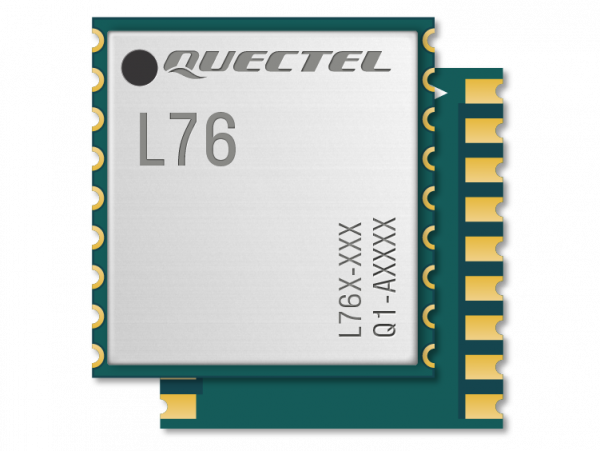
\includegraphics[width=.5\textwidth]{./Figures/QL76.png}
	\caption{Módulo Quectel L76\protect\footnotemark.}
	\label{fig:QL76}
\end{figure}
\footnotetext{Imagen tomada de: \url{https://www.quectel.com/product/gnss-l76}}

A continuación, se describen las características principales del módulo QL76 \citep{QL76}:

\begin{itemize}
    \item La configuración de constelación predeterminada es GPS+GLONASS.
    \item Admite interfaces de comunicación UART e I2C. 
    \item Ofrece diversos modos de funcionamiento que permiten la optimización del consumo de energía, a saber: GLP, AlwaysLocate™, Standby y Backup
    \item Tiene un consumo de energía extremadamente bajo.
\end{itemize}

 

\subsection{Módulo 4G}
\label{sec:SIMA7670SA}

Un transmisor/receptor 4G es un dispositivo terminal que permite la comunicación inalámbrica para dispositivos electrónicos a través de las redes de telefonía móvil de cuarta generación. Estos módulos facilitan la transmisión de datos, mensajes SMS, llamadas y conexión a internet a través de la infraestructura de redes móviles.

Para este trabajo se escogió el SoC (\textit{Sistem on Chip}) 4G SIMA7670SA con tecnología 4G. Soporta las bandas de frecuencia GSM y LTE-FDD. Está optimizado para casos de uso de IoT, diseñando bajo la especificación CAT-1. Puede oparar en condiciones difíciles, entre las que se pueden mencionar:
\begin{itemize} 
    \item Cobertura en lugares remotos.
    \item Interferencia por el fenómeno de \textit{handover}.
    \item Congestión de la red.
    \item Condiciones meteorológicas adversas. 
\end{itemize}

El SoC también integra el \textit{stack} de protocolos TCP/IP, MQTT. Este se escogió debido a que presenta buenas prestaciones en un tamaño compacto \citep{A7670SA}. 

\vspace{1cm}

\begin{figure}[htbp]
	\centering
	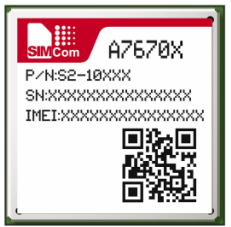
\includegraphics[width=.5\textwidth]{./Figures/A7670SA.jpg}
	\caption{Módulo SIM A7670SA\protect\footnotemark.}
	\label{fig:A7670SA}
\end{figure}
\footnotetext{Imagen tomada de: \url{https://www.simcom.com/product/A7670X.html}}

Las características principales de este SoC son: 

\begin{itemize}
    \item Frecuencias de trabajo: LTE-FDD(B1/B2/B3/B4/B5/B7/B8/B28/B66), GSM (850/900/1800/1900MHz).
    \item Soporta interfaces UART, USB, I2C y GPIO.
    \item Velocidad de descarga/carga en modo LTE de 10/5 Mbps.
    \item Velocidad de descarga/carga en modo GPRS/EDGE de 236.8/236.8 Kbps.
    \item consumo de corriente en modo LTE 3.8 mA.
    \item consumo de corriente en modo GSM 3.5 mA.
\end{itemize}

Para el presente trabajo, se utilizó el módulo A7670SA 4G LTE CAT1 MULTIBANDA GSM GPRS IOT (\textit{shield}) comercial basado en el SoC SIM A7670SA, debido a la facilidad para integrarlo al sistema general y que dispone de las interfaces de hardware necesarias para su interconexión con la ESP32, demás de su propio circuito de alimentación y un diseño fiable para evitar las interferencias electromagnéticas. Ver figura~\ref{fig:A7670SA_2}.

\begin{figure}[htbp]
	\centering
	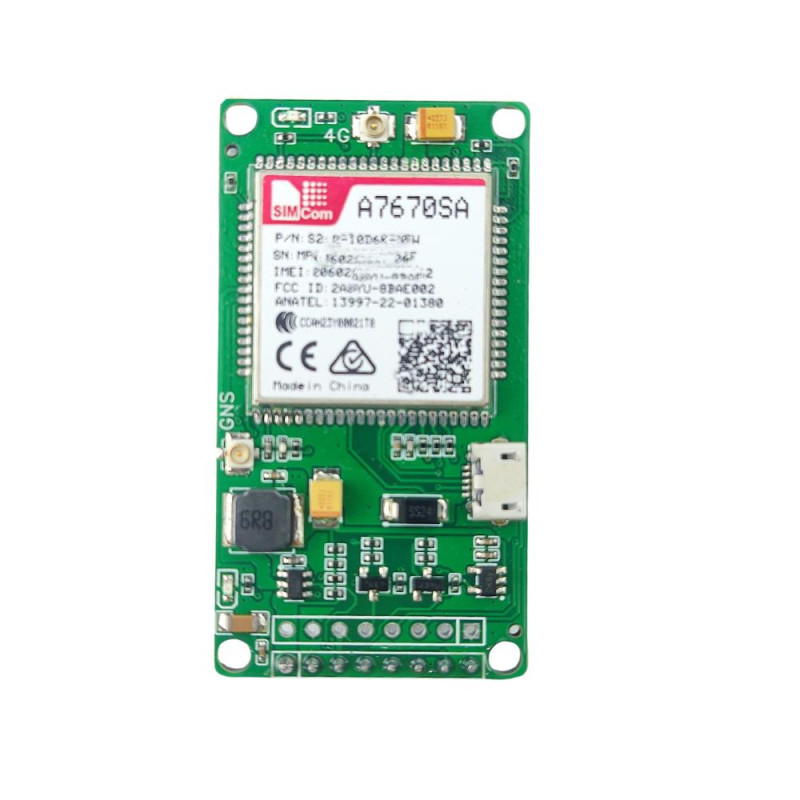
\includegraphics[width=.5\textwidth]{./Figures/A7670SA_Mod.jpg}
	\caption{Módulo A7670SA\protect\footnotemark.}
	\label{fig:A7670SA_2}
\end{figure}
\footnotetext{Imagen tomada de: \url{https://ssdielect.com/gsm-y-gprs-1/4872-a7670sa-sin-gps.html}}

\subsubsection{Antena Quectel YG0035AA}

Debido al requerimiento de conectarse, como mínimo, con dos constelaciones de satélites para obtener la posición geográfica, se debe utilizar una antena capaz de captar las frecuencias de transmisión de al menos dos constelaciones satelitales. Para este proyecto, se considera la antena Quectel YG0035AA. En la figura~\ref{fig:Antena} se observa la antena.

La antena está diseñada, según su fabricante, está diseñada con las características de alta eficiencia y excelente rendimiento. Soporta la recepción de señales de la constelación GPS y BeiDou (BD). Presenta las siguientes características eléctricas: 

\begin{itemize}
	\item Antena tipo activa.
	\item Rango de frecuencias de 1561 MHz a 1575 MHz.
	\item Impedancia de entrada de 50 ohm
	\item Ganancia entre 0.5 dBi y 1.4 dBi
	\item Polarización tipo RHCP. 
\end{itemize}

\begin{figure}[htbp]
	\centering
	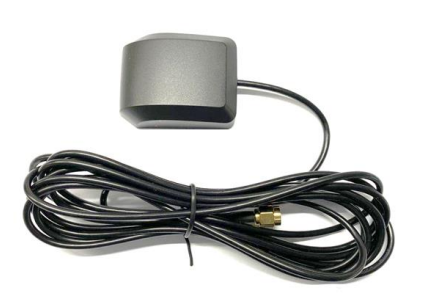
\includegraphics[width=.5\textwidth]{./Figures/Antena_Quectel_YG0035AA.png}
	\caption{Antena Quectel YG0035AA\protect\footnotemark.}
	\label{fig:Antena}
\end{figure}
\footnotetext{Imagen tomada de: \url{https://www.quectel.com/product/yg0035aa-gnss-active-magnetic-mount-antenna/}}



\subsection{Sistema operativo de tiempo real}
\label{sec:RTOS}

Un sistema operativo de tiempo real (RTOS, del inglés: Real-Time Operating System), es un tipo de sistema operativo diseñado específicamente para controlar y gestionar tareas de tiempo real en sistemas embebidos, como microcontroladores y sistemas integrados. La característica principal de un RTOS es que puede responder a eventos y ejecutar tareas de manera predecible y en un intervalo de tiempo garantizado.

El firmware que se implementó en este trabajo está basado en FreeRTOS™. En el apartado siguiente, se explica qué es y cuáles son las ventajas que se obtuvieron con su utilización. 

\subsubsection{FreeRTOS™}
\label{sec:FreeRTOS}

FreeRTOS™ es un sistema operativo de tiempo real de código abierto diseñado para sistemas embebidos y microcontroladores. Es apto para microcontroladores y microprocesadores pequeños \citep{FreeRTOS}. A continuación, se presentan las ventajas de haber implementado este sistema operativo en el trabajo.

\begin{itemize}
    \item Debido a que proporciona un kernel multitarea, permitió generar concurrencia entre tareas, como lo fueron la recepción y parseo de tramas GNSS, la transmisión de datos en tiempo real.  
    \item Gracias a la temporización precisa, se pudo asegurar la transmisión de datos de posicionamiento en tiempo real. 
    \item Permitió la gestión de la memoria y los periféricos UART del microcontrolador. De hecho, con FreeRTOS™, es posible gestionar todos los recursos del dispositivo con colas y semáforos. Al mismo tiempo, el kernel no representa una carga pesada para la capacidad de cómputo del microcontrolador utilizado. 
    \item Se pudo acceder a las ventajas de un RTOS de forma libre con la licencia MIT de FreeRTOS™.
    \item El código desarrollado es altamente portable, lo que permitirá escalar o transferir fácilmente el prototipo hacia otras plataformas. 
\end{itemize}



\subsection{Servicio web para mapas}
\label{sec:mapas_web}

Un servicio de mapas es un conjunto de herramientas y servicios de software que permiten que los mapas estén disponibles en la web. A menudo este es ofrecido por un proveedor especializado. 

Para este trabajo se creó una aplicación web basada en los servicios de la biblioteca para JavaScript Leaflet. Esta es de código abierto y ofrece todas las funciones cartográficas necesarias para la creación de aplicaciones que requieren el uso de mapas, como es el caso de la geolocalización.

En la tabla \ref{tabla:comparativa_api_mapas} se presenta una comparación entre tres bibliotecas que prestan herramientas para la creación de mapas en la web: 

\begin{table}[h]
    \centering
    \caption{Tabla comparativa de APIs de mapas.}
    \begin{tabular}{p{3cm} p{3cm} p{2.5cm} p{2.5cm} }
    \toprule
        \textbf{Característica}           & \textbf{Google Maps API}           & \textbf{Leaflet.js}               & \textbf{Carto.js} \\
        \midrule
        \textbf{Licencia}                & De pago, con un nivel gratuito limitado. & Open-source (BSD 2-clause License). & De pago, con un nivel gratuito limitado. \\
        
        \textbf{Facilidad de uso}        & Alta                               & Alta                              & Media \\
        
        \textbf{Documentación}           & Extensa y detallada.                & Buena, pero poco extensa. Complementa con muchos ejemplos. & Buena, orientada a usuarios con conocimientos en GIS \\
        
        \textbf{Soporte y Comunidad}     & Amplio soporte y gran comunidad.    & Gran comunidad open-source.         & Comunidad activa, pero reducida. \\
        
        \textbf{Capacidades de Mapa}     & Incluye vistas de satélite, terreno, y Street View. & Básico, pero extensible con plugins. & Enfocado en visualización de datos geoespaciales. \\
        
        \textbf{Personalización}           & Alta, mediante opciones y controles avanzados. & Muy alta, altamente personalizable con plugins. & Alta, especialmente en visualización de datos. \\
        
        \textbf{Rendimiento}             & Muy bueno, optimizado por Google.   & Muy bueno, especialmente en navegadores modernos. & Bueno, puede ser pesado con grandes conjuntos de datos. \\
        
        \textbf{Integración de Datos}    & Fácil integración con servicios de Google como Places, Routes, etc. & Necesita plugins adicionales para integración avanzada de datos. & Muy bueno para integración de datos geoespaciales y análisis. \\
        
        \textbf{Soporte para Móviles}    & Excelente, completamente responsive. & Muy bueno, compatible con dispositivos móviles. & Bueno, pero depende del tamaño de los datos. \\
        
        \textbf{Características Avanzadas} & Geocoding, Directions, Distance Matrix, Places API, etc. & Depende de plugins externos. & Análisis espacial avanzado, mapas temáticos, SQL API. \\
        
        \textbf{Facilidad de Integración} & Muy fácil con otros servicios de Google. & Fácil con bibliotecas JavaScript estándar. & Requiere conocimiento de GIS y SQL para máxima utilidad. \\
    \bottomrule
    \end{tabular}
    \label{tabla:comparativa_api_mapas}
\end{table}
 
\chapter{Diseño e implementación} % Main chapter title

\label{Chapter3} % Change X to a consecutive number; for referencing this chapter elsewhere, use \ref{ChapterX}


Este capítulo explica los componentes del sistema seleccionados y la descripción detallada de cada módulo de hardware y software desarrollados en el trabajo. Utilizando las definiciones y criterios descritos en capítulos anteriores, se comprende el diseño final del prototipo.

%----------------------------------------------------------------------------------------
%	SECTION 1
%----------------------------------------------------------------------------------------
\section{Diseño e implementación general del sistema}

El diseño e implementación general del sistema se subdividió en 3 partes: 

\begin{enumerate}
    \item Diseño e implementación del hardware.
    \item Diseño e implementación del firmware.
    \item Diseño e implementación de la interfaz web.
\end{enumerate}

A continuación, se describen cada una de estas partes.

%----------------------------------------------------------------------------------------
%	SECTION 2
%----------------------------------------------------------------------------------------
\section{Diseño e implementación de hardware}
\label{sec:dis_impl_hardware}

En esta sección, se describen las consideraciones de diseño del hardware del sistema. 

\subsection{Diseño del Hardware}

En la figura~\ref{fig:Arq_harware} se presenta la arquitectura del hardware desarrollado. Se incluyen todos los componentes descritos en las secciones anteriores. El sistema cuenta con 3 antenas correspondientes a la comunicación GNSS, 4G y Wi-Fi. 

Como parte de la interfaz humano-máquina, se cuenta con una pantalla LCD de 16x2, un botón para la indicación manual de estado ocupado/desocupado y dos pilotos que permiten visualizar el estado de ocupación actual. 

En el diagrama se pueden ver los protocolos de comunicación entre módulos, entre los que se destacan:

\begin{itemize}
    \item El protocolo UART para la comunicación entre el módulo 4G SIM A7670SA por el puerto UART 0 y el módulo  GNSS Quectel L76 por el puerto UART 1. 
    \item El protocolo I2C para la comunicación con la pantalla LCD. 
\end{itemize}

Se presenta una fuente de alimentación correspondiente a una batería de 12 VDC. Debido a que los componentes del sistema operan con tensiones diferentes, se hizo necesaria la implementación de circuitos adicionales. En el diagrama, estos circuitos se denominan <<Fuente>>. Estos suplen 2 niveles de tensión distintos: 

\begin{itemize}
    \item 3,3 VDC para el Quectel L76.
    \item 5 VDC para la ESP32, el módulo SIM A7670SA y la pantalla LCD.
\end{itemize}

\begin{figure}[htbp]
	\centering
	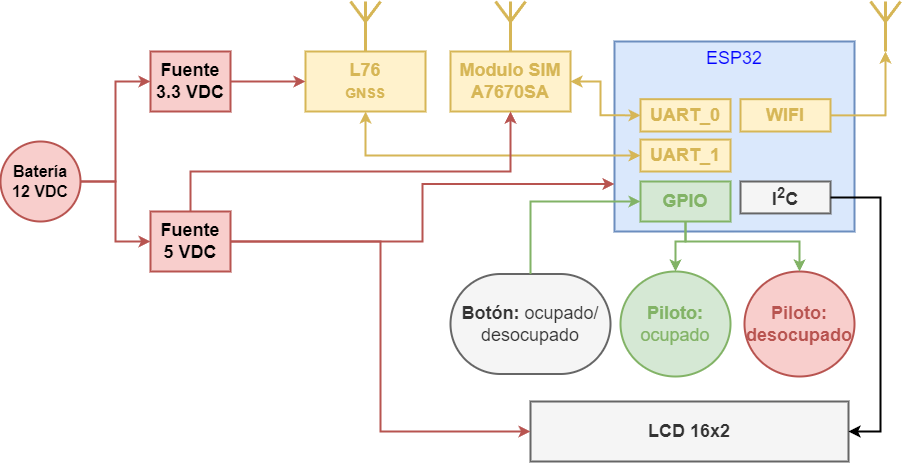
\includegraphics[width=1\textwidth]{./Figures/arquitectura_hardware_sistema.png}
	\caption{Arquitectura del hardware desarrollado.}
	\label{fig:Arq_harware}
\end{figure}



\subsection{Implementación del Hardware}

En la etapa de implementación del hardware, se trabajó en 2 placas de circuito impreso. 

\begin{enumerate}
    \item Placa base del sistema.
    \item Adaptador para el módulo Quectel L76.
\end{enumerate}



\subsubsection{Placa base del sistema}

La placa base se encargará de interconectar los módulos y periféricos principales del sistema. Por lo tanto, en el apéndice~\ref{AppendixA}, se presenta el circuito esquemático correspondiente a esta implementación. En esta se empleó el regulador MIC29302WU, con una configuración de ajuste por defecto en 5 VDC, para la alimentación de la ESP32, del módulo SIM A7670SA, la placa adaptador para el módulo Quectel L76 y la pantalla LCD. En la figura~\ref{fig:placa_base_2d} se puede apreciar el diseño final del PCB en un modelo de dos dimensiones. Además, en la figura~\ref{fig:placa_base_3d} se observa el modelo en tres dimensiones. 

Los componentes U1, U2 y H3, corresponden a las ranuras donde se conectan la ESP32 DevKit V4, el adaptador para el módulo Quectel L76, y el módulo SIM A7670SA. Las terminales marcadas con CN6 y CN7 permiten la conexión de los pilotos que indican la ocupación de la cava. Las terminales CN4 y CN5 corresponden a las conexiones de los botones de que dispondrá el operario de la cava para la indicación de la ocupación. Por otro lado, las terminales CN2 y CN3 corresponden a la interfaz I2C y la alimentación de la pantalla LCD, respectivamente. La terminal CN1 corresponde a la entrada de alimentación del sistema. Finalmente, las terminales CN9 y CN11 externalizan los pines GPI 34 y GPI 35, y GPIO 5 y GPIO 18 de la ESP32, respectivamente; esto para facilitar, en una etapa posterior, la agregación de nuevas funcionalidades. 

\begin{figure}[htbp]
	\centering
	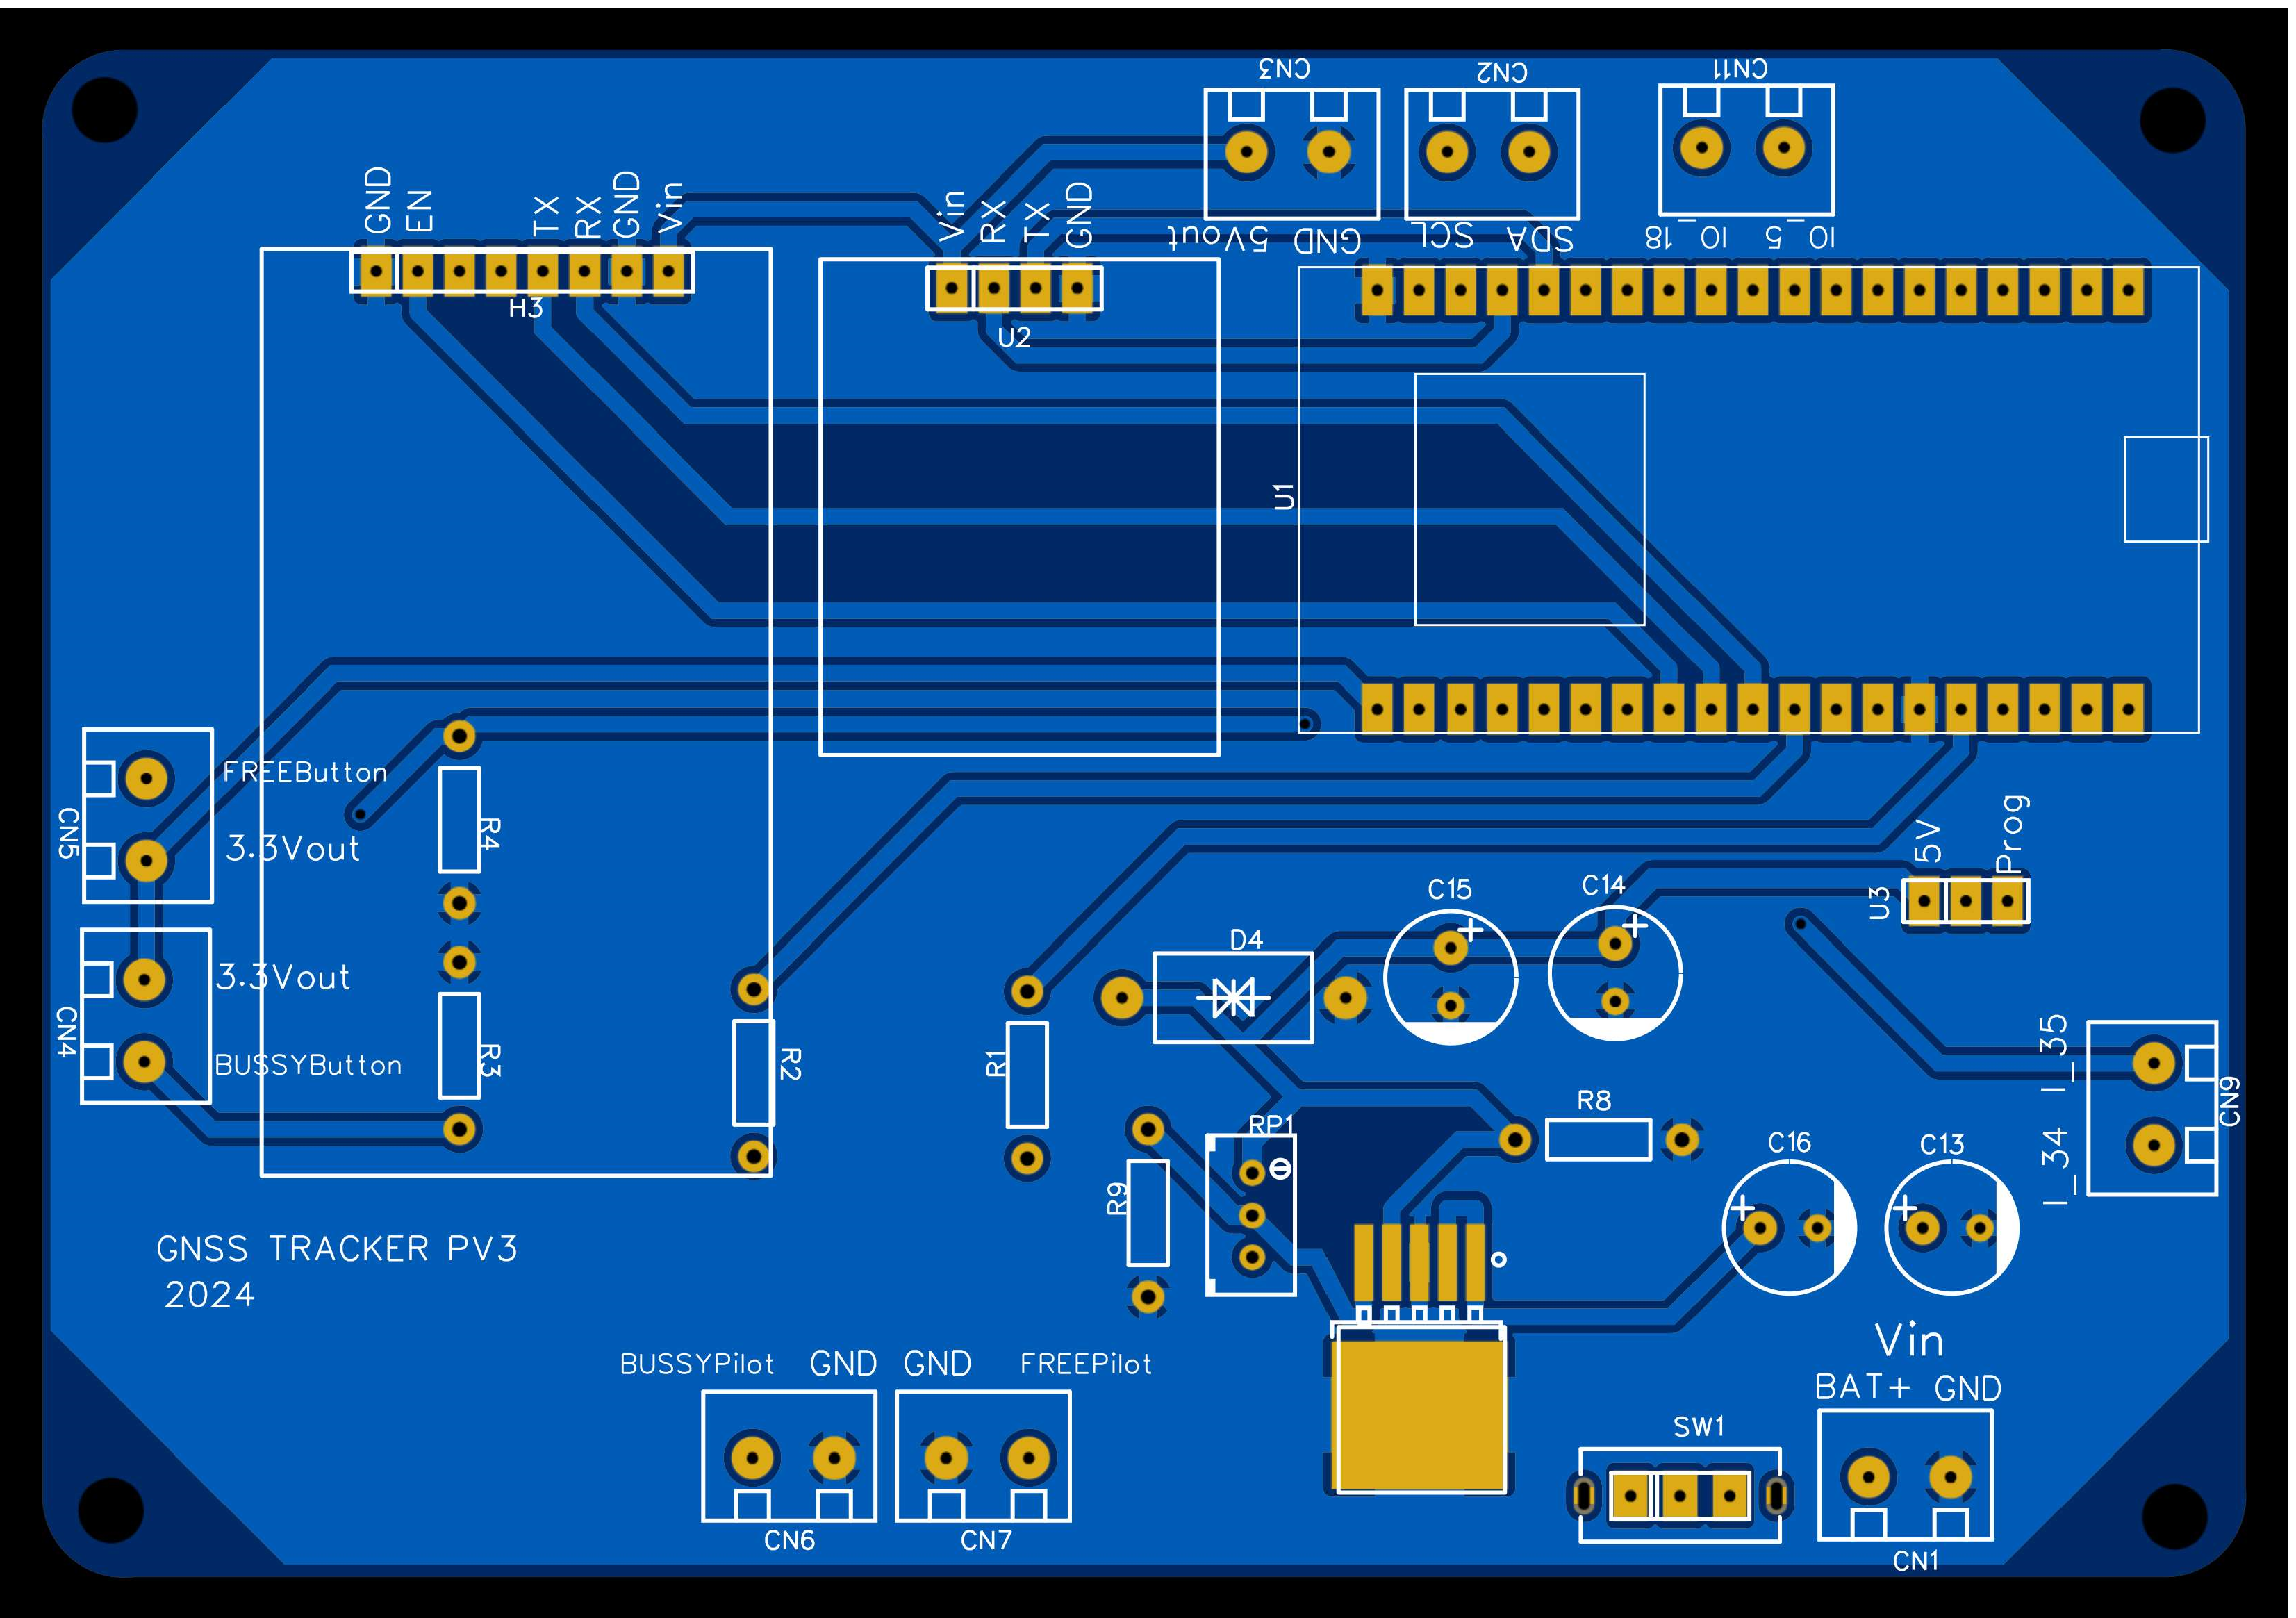
\includegraphics[width=.5\textwidth]{./Figures/PCB_TFE_Modelo_2D.png}
	\caption{Modelo 2D de la placa base del sistema.}
	\label{fig:placa_base_2d}
\end{figure}

\begin{figure}[htbp]
	\centering
	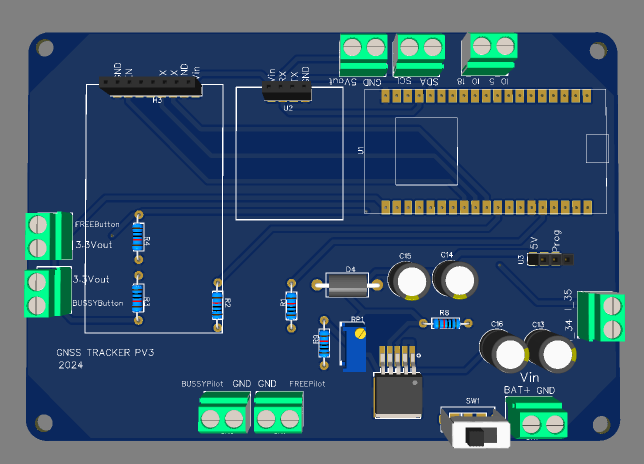
\includegraphics[width=.5\textwidth]{./Figures/PCB_TFE_Modelo_3D.png}
	\caption{Modelo 3D de la placa base del sistema.}
	\label{fig:placa_base_3d}
\end{figure}


\subsubsection{Adaptador para el módulo Quectel L76}

El circuito esquemático del adaptador L76 se encuentra en la figura~\ref{fig:adap_L76}. En este esquemático se puede observar la fuente de 3.3 VDC. Además, en la figura se presenta el circuito de entrada de alimentación, la conexión UART y la conexión entre el módulo y el microcontrolador ESP32.  

En las figuras~\ref{fig:adap_L76_2d} y~\ref{fig:adap_L76_3d}, se muestran los modelos 2D y 3D del circuito diseñado. 

\begin{figure}[htbp]
	\centering
	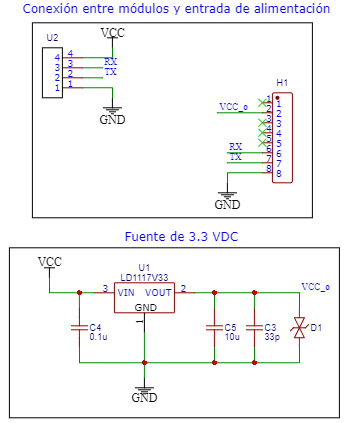
\includegraphics[width=.6\textwidth]{./Figures/QL76_Esquematico.png}
	\caption{Esquemático del adaptador L76.}
	\label{fig:adap_L76}
\end{figure}

\begin{figure}[htbp]
	\centering
	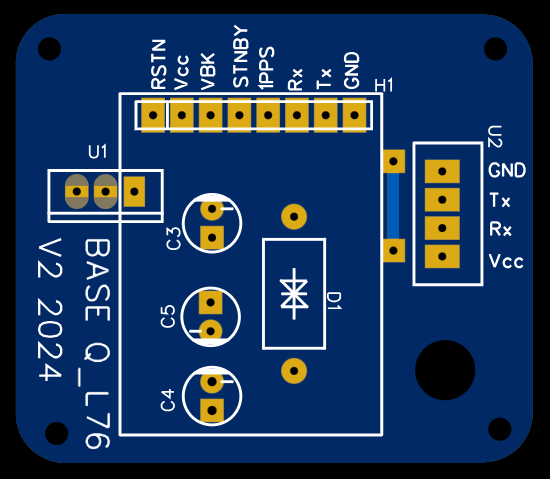
\includegraphics[width=.4\textwidth]{./Figures/QL76_modelo_2d_sup.png}
	\caption{Modelo 2D del adaptador L76.}
	\label{fig:adap_L76_2d}
\end{figure}

\begin{figure}[htbp]
	\centering
	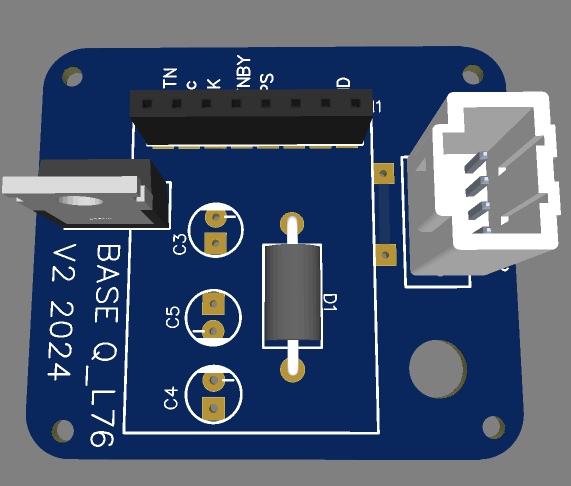
\includegraphics[width=.4\textwidth]{./Figures/QL76_modelo_3d_sup.png}
	\caption{Modelo 3D del adaptador L76.}
	\label{fig:adap_L76_3d}
\end{figure}



%----------------------------------------------------------------------------------------
%	SECTION 3
%----------------------------------------------------------------------------------------
\section{Diseño e implementación del firmware}

En esta sección se presentan las consideraciones de diseño y el proceso de implementación del firmware. 

\subsection{Diseño del firmware}

El propósito del firmware desarrollado es satisfacer los requerimientos de conectividad, administración del hardware e interfaz con el usuario. A continuación se describen las principales funcionalidades del firmware: 

\begin{enumerate}
 \item Realizar las funciones de conexión a Internet a través de la red celular, a través de la comunicación por comandos AT-UART con el módulo SIM A7670SA, para asegurar la conexión con el servidor utilizando el protocolo MQTT.
 \item Comunicación a través de tramas NMEA por el puerto UART con el módulo Quectel L76. Para la recepción e interpretación de la información de geolocalización de las constelaciones GPS y BeiDou.  
 \item Monitoreo de los botones de ocupación a través de interrupciones y visualización de los estados de ocupación a través de los pilotos. 
 \item Generación de interfaz visual a través de la comunicación I2C con la pantalla LCD 16x2. 
 \item Administración de la energía del sistema a través de los modos de bajo consumo de los módulos del sistema. 
 \item Administración de los recursos del microcontrolador a través de la implementación del sistema operativo en tiempo real FreeRTOS. 
\end{enumerate}

\subsubsection{Arquitectura del firmware}
\label{sec:arquitectura_firmware}

De acuerdo con lo planteado anteriormente, en la figura~\ref{fig:arq_firmware} se presenta un diagrama de componentes UML, que representa la arquitectura del sistema. 

En este diagrama (figura~\ref{fig:arq_firmware}) se representan como subsistemas (\textit{Subsystem}) los componentes de hardware como la ESP32, la pantalla LCD, el módulo 4G SIM A7670SA, los botones y los pilotos. Así mismo, se entienden como subsistemas los componentes de firmware proporcionados por el fabricante del microcontrolador, que corresponden a los drivers GPIO, UART y el bus I2C. Además, se hizo necesaria la implementación de una biblioteca propia para el control de la pantalla LCD a través del bus I2C.

De acuerdo con esto, los componentes del firmware se establecen en la ESP32, que corresponde al dispositivo programable encargado de realizar el control general del sistema. 

\begin{figure}[htbp]
	\centering
	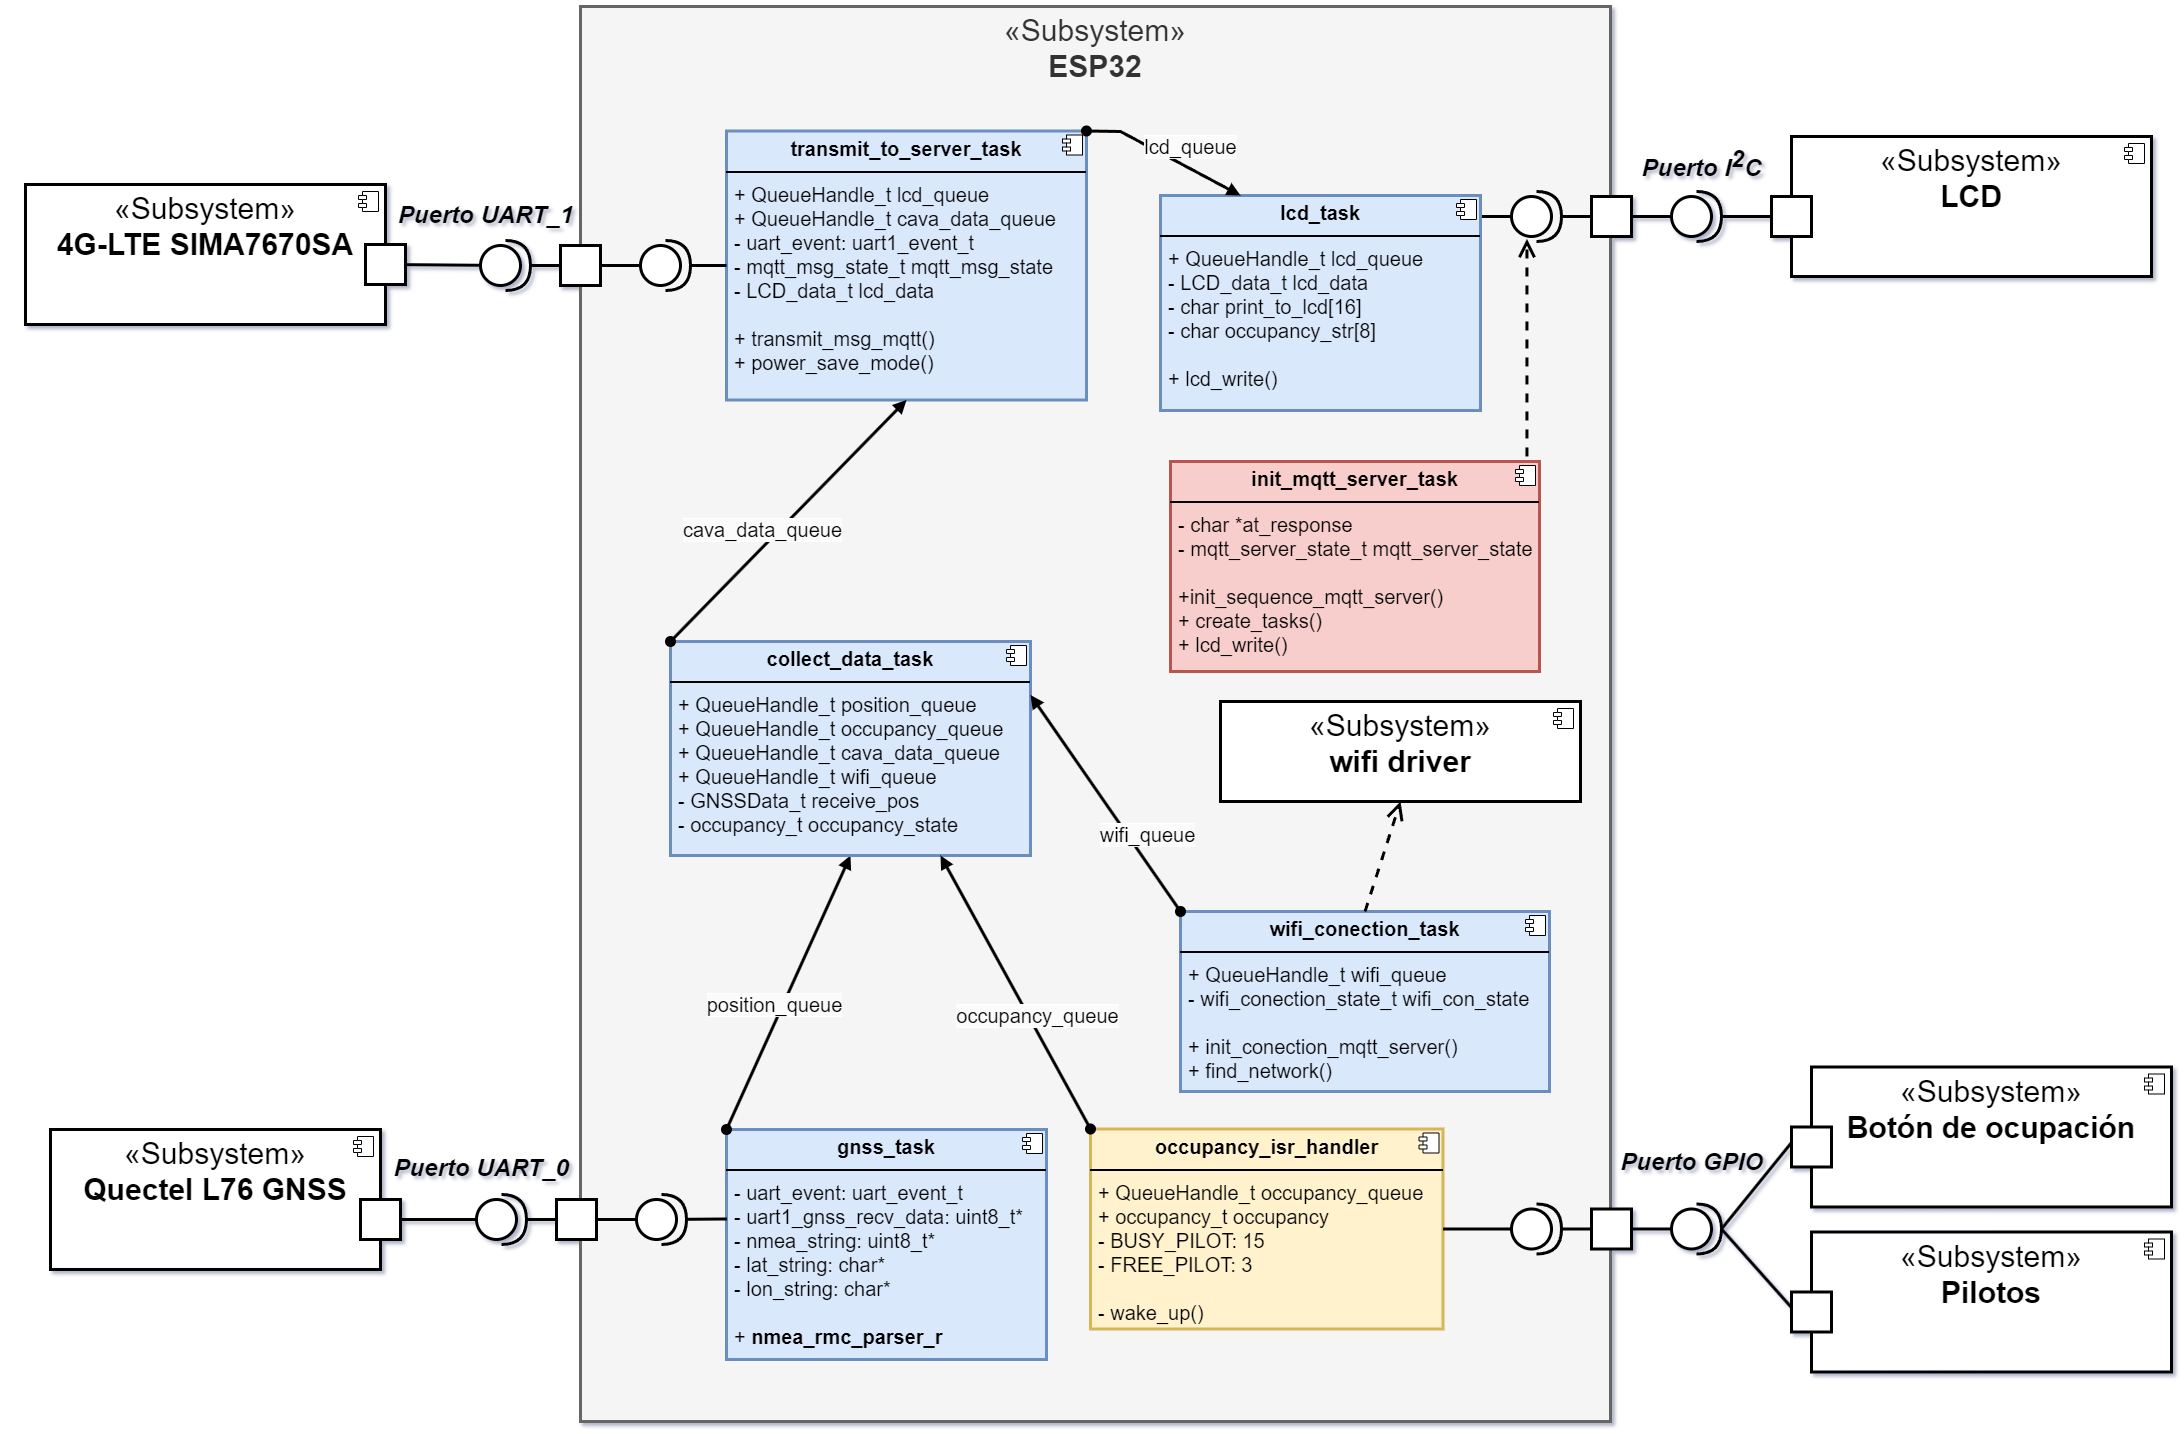
\includegraphics[width=1.1\textwidth]{./Figures/Arquitectura_firmware_TFE_GNSS.png}
	\caption{Arquitectura del firmware.}
	\label{fig:arq_firmware}
\end{figure}

En el diagrama de la figura~\ref{fig:arq_firmware} se presentan las los componentes de firmware más relevantes del sistema y la forma en que interactúan entre ellos. A continuación, se describe la funcionalidad d ecada componente del firmware:

\begin{enumerate}
	\item El firmware inicia con la tarea \textit{init\_mqtt\_server\_task()}, resaltada con color rojo, la cual se encarga de tres funciones primordiales: realizar la inicialización de los servicios MQTT que proporciona el módulo 4G (SIM A7670SA), realizar la conexión con el servidor remoto y, si todo sale bien, desencadena la creación de las demás tareas del sistema. Esta tarea utiliza líneas de comandos AT para comunicarse con el módulo 4G.
	
	\item Tarea \textit{collect\_data\_task()}, se encarga de recibir a través de colas, la información relacionada con la ocupación y la posición de la cava, dicha información proveniente de la tarea \textit{gnss\_task()} y del manejador de interrupciones \textit{occupancy\_isr\_handler()}, respectivamente. Cuando esta tarea obtiene la información mencionada, las transmite a la tarea \textit{transmit\_to\_server\_task()}, a través de la cola \textit{cava\_data\_queue}.
	
	\item Manejador de interrupción \textit{occupancy\_isr\_handler()}, resaltada con color amarillo, es la función que se ejecuta siempre que ocurra una interrupción debida a los botones de ocupación de la cava, a saber, ocupado-desocupado. Este manejador de interrupción detecta qué botón se presionó, y comunica a la tarea \textit{collect\_data\_task()} el estado de ocupación, a través de la cola \textit{occupancy\_queue}. Además, esta tarea genera una acción de \textit{wakeup} del sistema cuando se encuentra en modo ahorro de energía. 	
	
	\item Tarea \textit{gnss\_task()}, se encarga primordialmente de detectar la recepción de una trama NMEA del tipo GNRMC, lo que asegura que la posición ha sido calculada con señales de dos o más constelaciones satelitales; en este caso, GPS y BeiDou. La detección de tramas se realiza a través de interrupciones del módulo UART de la ESP32. Esta tarea descarta todas las tramas que no sean compatibles con el estándar NMEA y todas las que no sean del tipo GNRMC. Además, se encarga de la extracción de la información de las tramas RMC a través de la función \textit{nmea\_rmc\_parser\_r()}. Esta última es una implementación de tipo \textit{thread-safe} para asegurar la compatibilidad con FreeRTOS, ya que permite la multitarea. Además, comunica la posición actual a la tarea \textit{collect\_data\_task()}, a través de la cola \textit{position\_queue}. Por último, esta tarea verifica si la posición no ha cambiado en los últimos 5 minutos, en caso de no cambiar, colocará al sistema completo en modo ahorro de energía. 
		
	\item Tarea \textit{transmit\_to\_server\_task()}, se encarga de ejecutar la secuencia de transmisión de datos a través del protocolo MQTT, con el módulo 4G. La comunicación entre microcontrolador y el módulo se realiza a través de comandos AT. Esta tarea recibe los datos provenientes de la tarea \textit{collect\_data\_task()}, los transmite con la función \textit{transmit\_msg\_mqtt()}. Al finalizar, construye un paquete de información con los datos de ocupación, posición y resultado de la transmisión MQTT, para ser transferido a través de la cola \textit{lcd\_queue} hacia la tarea \textit{lcd\_task()}. 
		
	\item Tarea \textit{lcd\_task()} se encarga de administrar adecuadamente el acceso a los recursos de la pantalla LCD, para evitar sobrescritura o pérdida de información relevante que deba ser mostrada a través de la pantalla LCD. 
\end{enumerate}



\subsection{Implementación del firmware}
\label{sec:implementacion_firmware}

El firmware se implementó en el \textit{framework} ESP-IDF desarrollado por la empresa ESPRESSIF, para las series de SoCs ESP32, ESP32-S y ESP32-C. Este \textit{framework} proporciona un SDK apto para el desarrollo de cualquier aplicación genérica en estas plataformas, a partir de lenguajes de programación C y C++. Además, está optimizado para para aplicaciones de Internet de las Cosas (IoT, del inglés \textit{Internet of Things}). 

También se utilizó el entorno de desarrollo (IDE) \textit{PlatformIO}, que corre como una extensión nativa en el IDE de \textit{Visual Studio Code}. \textit{PlatformIO} permite usar todas las funcionalidades de ESP-IDF de una manera fiable y ágil, sin enmascarar funcionalidades o configuraciones avanzadas del \textit{framework}. Además, permite ejecutar las versiones mas estables de ESP-IDF, proporciona soporte por la comunidad de desarrolladores, es multiplataforma y de software libre. 

Para la implementación del firmware se utilizó el lenguaje de programación C y se implementó el sistema operativo en tiempo real FreeRTOS. Una ventaja importante que ofrece ESP-IDF es que está desarrollado sobre FreeRTOS, por tanto, el firmware se ejecuta nativamente en este. 

\subsubsection{Flujo general del firmware}

Gracias a la implementación en FreeRTOS, el firmware tiene la capacidad de ejecutar multitarea. El flujo general del programa se muestra en las figuras \ref{fig:flujo_firmware_1}, \ref{fig:flujo_firmware_2} y \ref{fig:flujo_firmware_3}. Como se puede ver en dicho diagrama y en el diagrama de la arquitectura (ver figura \ref{fig:arq_firmware}), las diferentes tareas se ejecutan una independiente de la otra. Sin embargo, existe un flujo de información que se sucede de una tarea a otra. Como mecanismo de comunicación entre tareas, se usan las colas. Este comportamiento del firmware es relevante desde el punto de vista en que el sistema puede estar recibiendo, procesando y transmitiendo datos de posicionamiento de manera casi concurrente. 

\begin{figure}
	\centering
	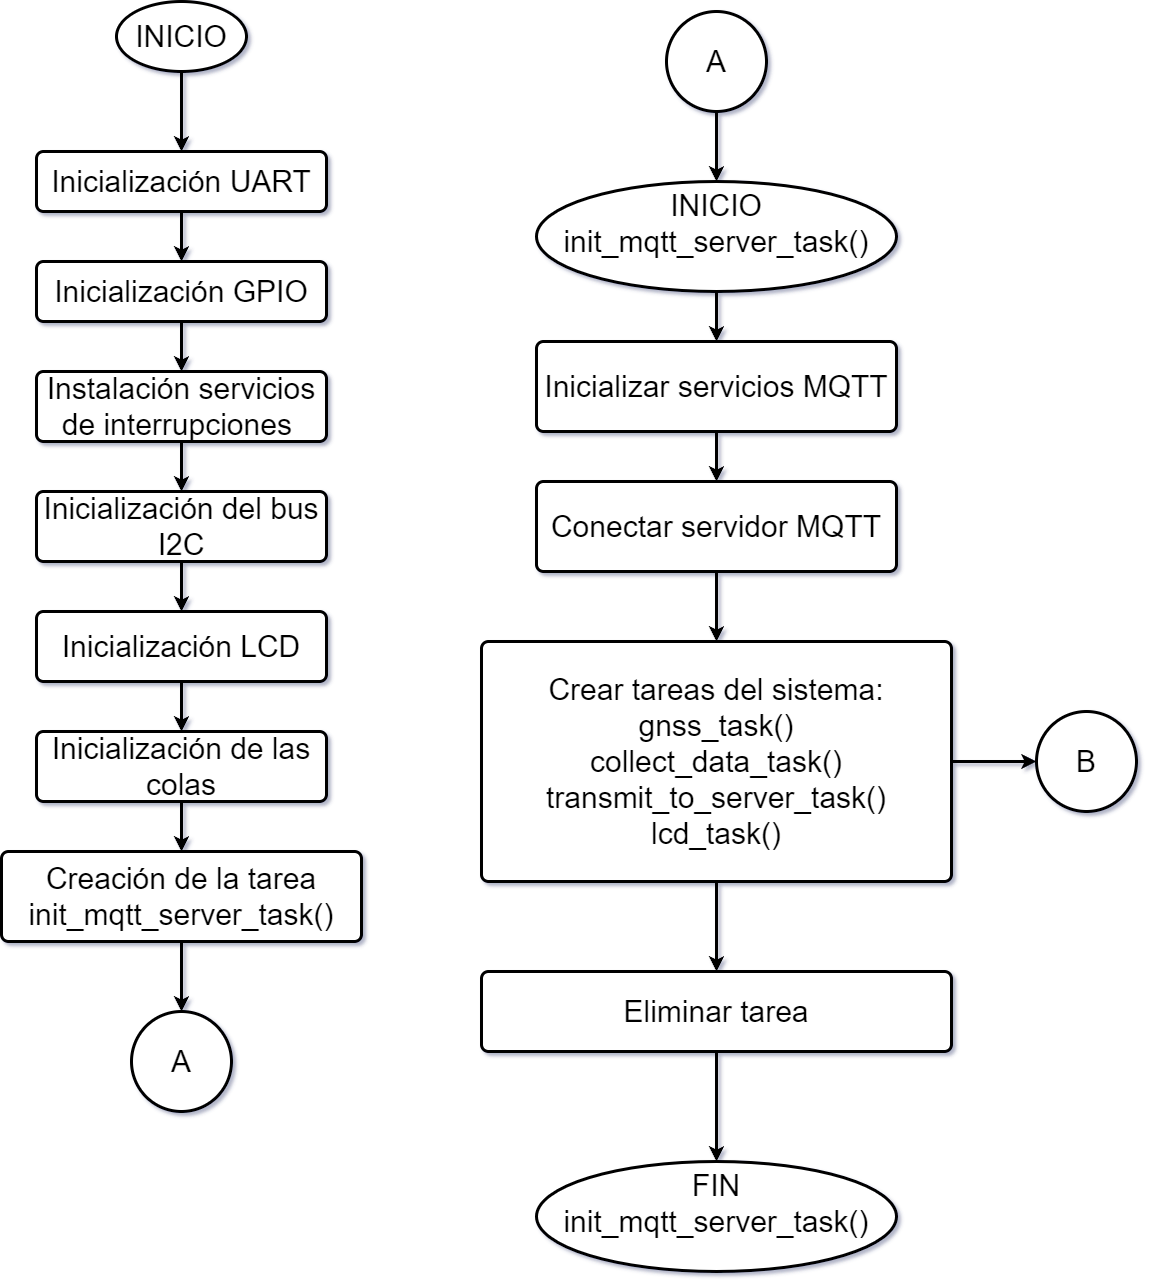
\includegraphics[width=.8\textwidth]{./Figures/Diagrama_flujo_firmware_TFE_CESE_Part_1.png}
	\caption{Diagrama de flujo del firmware (parte 1).}
	\label{fig:flujo_firmware_1}
\end{figure}

\begin{figure}
	\centering
	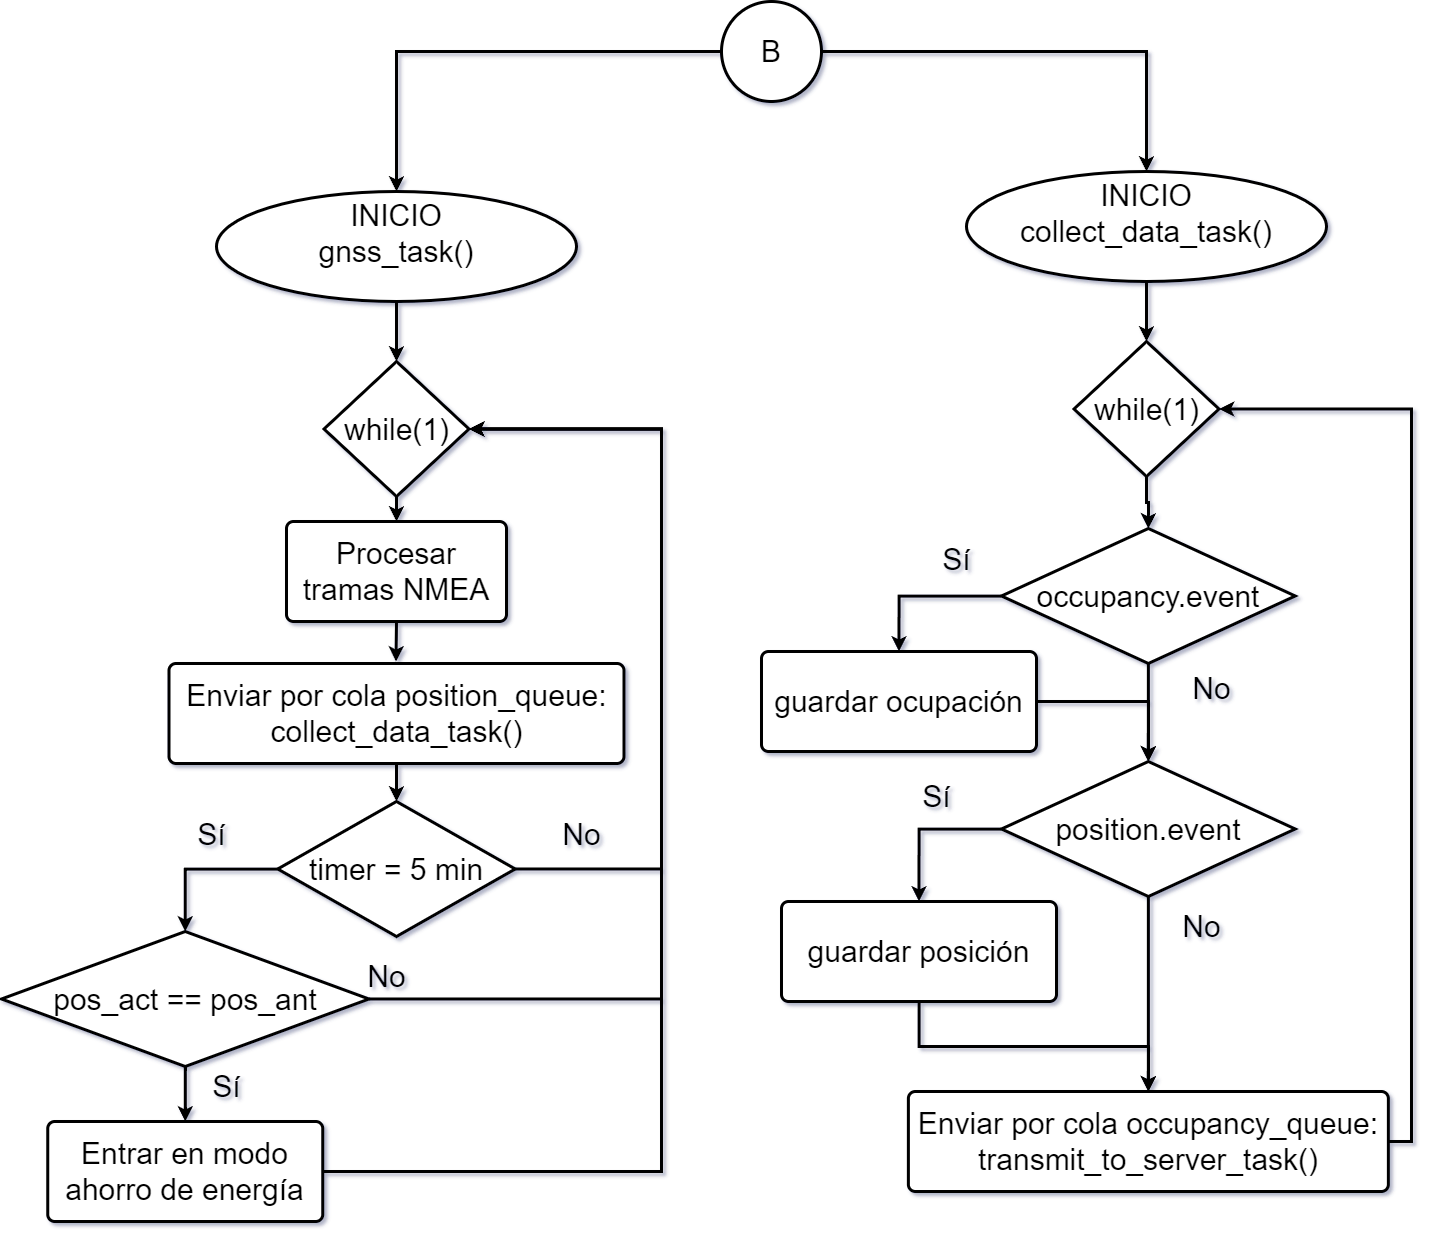
\includegraphics[width=.8\textwidth]{./Figures/Diagrama_flujo_firmware_TFE_CESE_Part_2.png}
	\caption{Diagrama de flujo del firmware (parte 2).}
	\label{fig:flujo_firmware_2}
\end{figure}

\begin{figure}
	\centering
	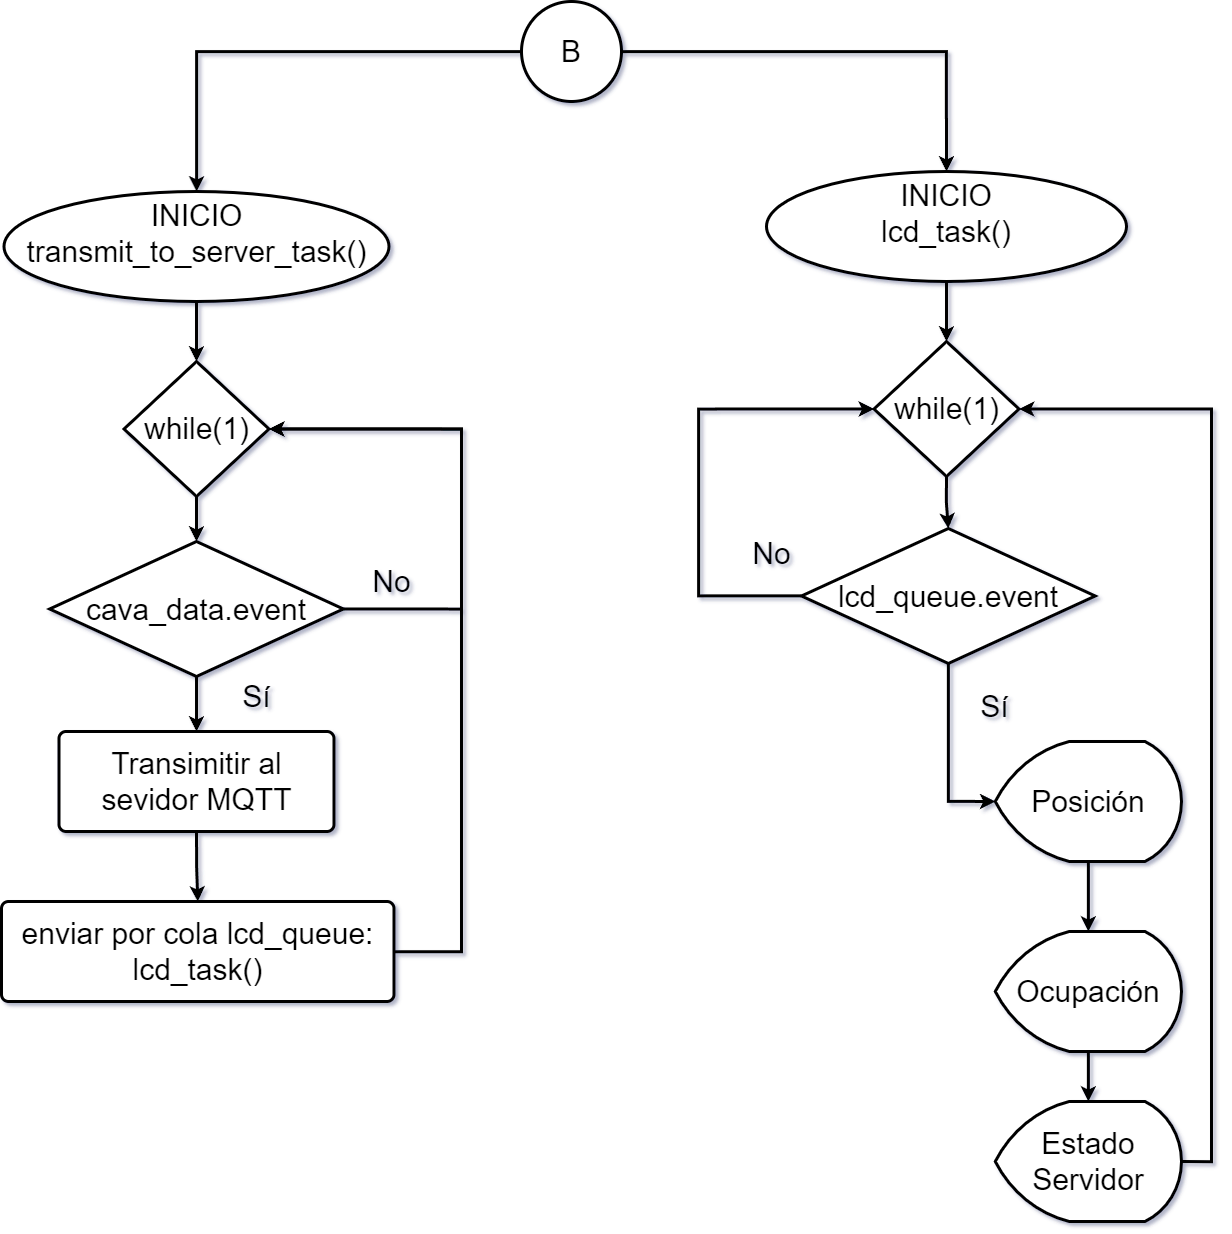
\includegraphics[width=.8\textwidth]{./Figures/Diagrama_flujo_firmware_TFE_CESE_Part_3.png}
	\caption{Diagrama de flujo del firmware (parte 3).}
	\label{fig:flujo_firmware_3}
\end{figure}


\subsubsection{Implementación de las tareas del sistema}

En los códigos, \ref{cod:init_mqtt_server_task}, \ref{cod:gnss_task}, \ref{cod:occupancy_isr_handler}, \ref{cod:collect_data_task}, \ref{cod:transmit_to_server_task} y \ref{cod:lcd_task} se presenta la implementación en pseudocódigo de cada una de las tareas principales del firmware. 


\begin{lstlisting}[label=cod:init_mqtt_server_task, caption=Pseudocódigo de la función init\_mqtt\_server\_task().] 

init_mqtt_server_task()
{
	while ("READY" == SIM_A7670SA)
		Esperar
	Inicalizar servicios MQTT en SIM_A7670SA
	while (4 == intentos)
		Conectar con servidor MQTT en la nube
		if ("OK" == Conexion_Servidor)
			Crear tareas: 
				gnss_task()
				collect_data_task()
				transmit_to_server_task()
				lcd_task()
			Eliminar: init_mqtt_server_task
			break
		else
			Reportar por LCD: Falla conexion servidor
			Eliminar: init_mqtt_server_task
}

\end{lstlisting}

 


\begin{lstlisting}[label=cod:gnss_task, caption=Pseudocódigo de la función gnss\_task().] 

gnss_task()
{
	while (1)
		if (DATA == envento_UART_0)
			Procesar trama: 
				posicion_actual = nmea_rmc_parser_r()
			Enviar por cola position_queue: posicion_actual
			if (Temporizar 5)
				if (posicion_anterior == posicion_actual)
					sleep_mode: Modulo_celular
					sleep_mode: Modulo_GNSS
					sleep_mode: ESP32
					
		posicion_anterior = posicion_actual
}

\end{lstlisting}

 


\begin{lstlisting}[label=cod:occupancy_isr_handler, caption=Pseudocódigo de la función occupancy\_isr\_handler().] 

occupancy_isr_handler()
{
	Capturar boton presionado
	switch (bonton)
		case boton_libre: 
			Setear los pilotos como libre
			Enviar por cola occupancy_queue: "Libre"
		
		case boton_ocupado:
			Setear los pilotos como ocupado
			Enviar por cola occupancy_queue: "Ocupado"	
}

\end{lstlisting}

 

\begin{lstlisting}[label=cod:collect_data_task, caption=Pseudocódigo de la función collect\_data\_task().] 

collect_data_task()
{
	while (1)
		if (DATA == occupancy_queue.event)
			datos_cava.occupancy = occupancy
			
		if (DATA == position_queue.event)
			datos_cava.position = position
		
		Enviar por cola cava_data_queue: datos_cava		
}

\end{lstlisting}

 

\begin{lstlisting}[label=cod:transmit_to_server_task, caption=Pseudocódigo de la función transmit\_to\_server\_task().] 

transmit_to_server_task()
{
	posicion_anterior
	while (1)
		if (DATA == cava_data_queue.event)
			Transmitir al servidor MQTT: 
				transmision_state = transmit_msg_mqtt()
			Enviar por cola lcd_queue: cava_data+transmision_state
}

\end{lstlisting}

 

\begin{lstlisting}[label=cod:lcd_task, caption=Pseudocódigo de la función lcd\_task().] 

lcd_task()
{
	while (1)
		if (DATA == lcd_queue.event)
			Escribir_LCD: position.lat
			Escribir_LCD: position.long
			Escribir_LCD: position.time
			Escribir_LCD: position.val // Validez de la posicion
			Escribir_LCD: occupancy
			Escribir_LCD: server_state
}

\end{lstlisting}



\subsubsection{Otros componentes del firmware}

Además de las tareas y funciones descritas en la sección \ref{fig:arq_firmware}, fue necesario implementar varios componentes de firmware. Sin embargo, por ser los más relevantes, se mencionan los siguientes:

\begin{enumerate}
	\item Un driver para el manejo de la pantalla \textit{LCD RGB Backlight} de 16x2 que se llamó \textit{lcd\_i2c\_grove.h}. Esta pantalla presenta interfaz de comunicación I2C, para reducir la cantidad de pines utilizados por el microcontrolador. Este driver presenta las funciones descritas en el código \ref{lst:driver_lcd}.
	
	\item Una función para inicializar los servicios MQTT en el módulo SIM A7670SA y conectarse al servidor en la nube, que se llamó \textit{init\_sequence\_mqtt\_server()}. Esta función implementa comandos AT específicos para el módulo en mención. Retorna el estado de conexión con el servidor o en su defecto los errores encontrados en el proceso. En el código \ref{cod:init_sequence_mqtt_server} se muestra el pseudocódigo que describe su funcionamiento.
	
	\item Una función para encapsular la funcionalidad de transmitir al servidor MQTT una vez se ha establecido la conexión. Esta es \textit{transmit\_msg\_mqtt()}. Esta función implementa comandos AT específicos del módulo SIM A7670SA y retorna el estado de transmisión del mensaje. En el código \ref{cod:transmit_msg_mqtt} se muestra el pseudocódigo que describe su funcionamiento.
	
	\item Una función que permite extraer la información de las cadenas tipo GNRMC recibidas por el módulo Quectel L76. Esta es una función de tipo \textit{thread-safe} para facilitar la multitarea, que se nombró como \textit{nmea\_rmc\_parser\_r()}. En el código \ref{cod:nmea_rmc_parser_r} se muestra el pseudocódigo que describe su funcionamiento.
\end{enumerate}


\begin{lstlisting}[label={lst:driver_lcd}, caption={Funciones principales del driver LCD.}] 

/**
 * @brief Esta funcion incializa las funcionalidades I2C y la configuracion de escritura de la pantalla
 */
void lcd_init();

/**
 * @brief Esta funcion escribe en la pantalla LCD el texto deseado.
 * 
 * @param row: Columna desde la cual se inica la escritura
 * @param column: Fila sobre la cual se desea escribir
 * @param str: Texto que se desea escribir
 */
void lcd_write(uint8_t row, uint8_t column, char *str);

/**
 * @brief Esta funcion limpia o borra todos los caracteres de la pantalla LCD.
 */
void lcd_clear();

/**
 * @brief Esta funcion cambia el color de fondo de la pantalla LCD segun el modelo de color RGB.
 * 
 * @param r: valor para cantidad de color rojo.
 * @param g: valor para cantidad de color verde.
 * @param b: valor para cantidad de color azul.
 */
void lcd_set_RGB(unsigned char r, unsigned char g, unsigned char b);

\end{lstlisting}

 


\begin{lstlisting}[label=cod:init_sequence_mqtt_server, caption=Pseudocódigo de la función init\_sequence\_mqtt\_server().] 

init_sequence_mqtt_server(uart_event_t uart1_event, char * at_response)
{
  Enviar AT: iniciar el servicio MQTT
  if ("OK" == respuesta)
      Enviar AT: adquirir cliente MQTT
      if ("OK" == respuesta)
          Enviar AT: conectar con servidor MQTT
	      if ("OK" == respuesta)
	          return: MQTT_SERVER_OK
	      else 
	          return: MQTT_FAIL_INIT_SERVER
      else
          return: MQTT_FAIL_ADQ_CLIENT
  else
      return: MQTT_FAIL_INIT_SERVICE	
}

\end{lstlisting}
 




\begin{lstlisting}[label=cod:transmit_msg_mqtt, caption=Pseudocódigo de la función init\_sequence\_mqtt\_server().] 

transmit_msg_mqtt(char * mqtt_payload, char * topic, uart_event_t uart1_event, char * at_response)
{
	Enviar AT: configurar topic
	if ("OK" == respuesta)
		Enviar AT: cargar payload
		if ("OK" == respuesta)
			Enviar AT: publicar
			if ("OK" == respuesta)
				return: MQTT_MSG_OK
			else
				return: MQTT_MSG_FAIL
		else
			return: MQTT_MSG_FAIL
	else
		return: MQTT_TOPIC_FAIL
}

\end{lstlisting}

 


\begin{lstlisting}[label=cod:nmea_rmc_parser_r, caption=Pseudocódigo de la función nmea\_rmc\_parser\_r().] 

nmea_rmc_parser_r(char *nmeaString, GNSSData_t *gnssData)
{
	Verificar trama inicia con "$"
	if ("$" == token_0)
		Dividir trama en tokens por ","
		Verificar que el primer token sea "GNRMC"
		if("GNRMC" == token_1)
			time = token_2 
			if("A" == token_3)
				latitud = convertir_DMS_to_DD(token_4, token_5)
				longitud = convertir_DMS_to_DD(token_6, token_7)
			else
				return: NMEA_NO_VALID			
			 
		else
			return: NMEA_NO_RMC
	else
		return: NMEA_NO_VALID
}

\end{lstlisting}




%----------------------------------------------------------------------------------------
%	SECTION 4
%----------------------------------------------------------------------------------------
\section{Diseño e implementación de la interfaz web}

\subsection{Diseño de la interfaz web}


\subsection{Implementación de la interfaz web}





















\begin{comment}

\definecolor{mygreen}{rgb}{0,0.6,0}
\definecolor{mygray}{rgb}{0.5,0.5,0.5}
\definecolor{mymauve}{rgb}{0.58,0,0.82}

%%%%%%%%%%%%%%%%%%%%%%%%%%%%%%%%%%%%%%%%%%%%%%%%%%%%%%%%%%%%%%%%%%%%%%%%%%%%%
% parámetros para configurar el formato del código en los entornos lstlisting
%%%%%%%%%%%%%%%%%%%%%%%%%%%%%%%%%%%%%%%%%%%%%%%%%%%%%%%%%%%%%%%%%%%%%%%%%%%%%
\lstset{ %
  backgroundcolor=\color{white},   % choose the background color; you must add \usepackage{color} or \usepackage{xcolor}
  basicstyle=\footnotesize,        % the size of the fonts that are used for the code
  breakatwhitespace=false,         % sets if automatic breaks should only happen at whitespace
  breaklines=true,                 % sets automatic line breaking
  captionpos=b,                    % sets the caption-position to bottom
  commentstyle=\color{mygreen},    % comment style
  deletekeywords={...},            % if you want to delete keywords from the given language
  %escapeinside={\%*}{*)},          % if you want to add LaTeX within your code
  %extendedchars=true,              % lets you use non-ASCII characters; for 8-bits encodings only, does not work with UTF-8
  %frame=single,	                % adds a frame around the code
  keepspaces=true,                 % keeps spaces in text, useful for keeping indentation of code (possibly needs columns=flexible)
  keywordstyle=\color{blue},       % keyword style
  language=[ANSI]C,                % the language of the code
  %otherkeywords={*,...},           % if you want to add more keywords to the set
  numbers=left,                    % where to put the line-numbers; possible values are (none, left, right)
  numbersep=5pt,                   % how far the line-numbers are from the code
  numberstyle=\tiny\color{mygray}, % the style that is used for the line-numbers
  rulecolor=\color{black},         % if not set, the frame-color may be changed on line-breaks within not-black text (e.g. comments (green here))
  showspaces=false,                % show spaces everywhere adding particular underscores; it overrides 'showstringspaces'
  showstringspaces=false,          % underline spaces within strings only
  showtabs=false,                  % show tabs within strings adding particular underscores
  stepnumber=1,                    % the step between two line-numbers. If it's 1, each line will be numbered
  stringstyle=\color{mymauve},     % string literal style
  tabsize=2,	                   % sets default tabsize to 2 spaces
  title=\lstname,                  % show the filename of files included with \lstinputlisting; also try caption instead of title
  morecomment=[s]{/*}{*/}
}

Se puede agregar código o pseudocódigo dentro de un entorno lstlisting con el siguiente código:

\begin{verbatim}
\begin{lstlisting}[caption= "un epígrafe descriptivo"]
	las líneas de código irían aquí...
\end{lstlisting}
\end{verbatim}

A modo de ejemplo:

\begin{lstlisting}[label=cod:vControl,caption=Pseudocódigo del lazo principal de control.]  % Start your code-block

#define MAX_SENSOR_NUMBER 3
#define MAX_ALARM_NUMBER  6
#define MAX_ACTUATOR_NUMBER 6

uint32_t sensorValue[MAX_SENSOR_NUMBER];		
FunctionalState alarmControl[MAX_ALARM_NUMBER];	//ENABLE or DISABLE
state_t alarmState[MAX_ALARM_NUMBER];						//ON or OFF
state_t actuatorState[MAX_ACTUATOR_NUMBER];			//ON or OFF

void vControl() {

	initGlobalVariables();
	
	period = 500 ms;
		
	while(1) {

		ticks = xTaskGetTickCount();
		
		updateSensors();
		
		updateAlarms();
		
		controlActuators();
		
		vTaskDelayUntil(&ticks, period);
	}
}
\end{lstlisting}

\end{comment}


% Chapter Template

\chapter{Ensayos y resultados} % Main chapter title

\label{Chapter4} % Change X to a consecutive number; for referencing this chapter elsewhere, use \ref{ChapterX}

%----------------------------------------------------------------------------------------
%	SECTION 1
%----------------------------------------------------------------------------------------

\section{Pruebas funcionales del hardware}
\label{sec:pruebasHW}

La idea de esta sección es explicar cómo se hicieron los ensayos, qué resultados se obtuvieron y analizarlos.
 
% Chapter Template

\chapter{Conclusiones} % Main chapter title

\label{Chapter5} % Change X to a consecutive number; for referencing this chapter elsewhere, use \ref{ChapterX}


%----------------------------------------------------------------------------------------

%----------------------------------------------------------------------------------------
%	SECTION 1
%----------------------------------------------------------------------------------------

\section{Conclusiones generales }

La idea de esta sección es resaltar cuáles son los principales aportes del trabajo realizado y cómo se podría continuar. Debe ser especialmente breve y concisa. Es buena idea usar un listado para enumerar los logros obtenidos.

Algunas preguntas que pueden servir para completar este capítulo:

\begin{itemize}
\item ¿Cuál es el grado de cumplimiento de los requerimientos?
\item ¿Cuán fielmente se puedo seguir la planificación original (cronograma incluido)?
\item ¿Se manifestó algunos de los riesgos identificados en la planificación? ¿Fue efectivo el plan de mitigación? ¿Se debió aplicar alguna otra acción no contemplada previamente?
\item Si se debieron hacer modificaciones a lo planificado ¿Cuáles fueron las causas y los efectos?
\item ¿Qué técnicas resultaron útiles para el desarrollo del proyecto y cuáles no tanto?
\end{itemize}


%----------------------------------------------------------------------------------------
%	SECTION 2
%----------------------------------------------------------------------------------------
\section{Próximos pasos}

Acá se indica cómo se podría continuar el trabajo más adelante.
 

%----------------------------------------------------------------------------------------
%	CONTENIDO DE LA MEMORIA  - APÉNDICES
%----------------------------------------------------------------------------------------

\appendix % indicativo para indicarle a LaTeX los siguientes "capítulos" son apéndices

% Incluir los apéndices de la memoria como archivos separadas desde la carpeta Appendices
% Descomentar las líneas a medida que se escriben los apéndices

% Appendix A

\chapter{Esquemáctico de la placa base del sistema} % Main appendix title
\label{AppendixA} % For referencing this appendix elsewhere, use \ref{AppendixA}



%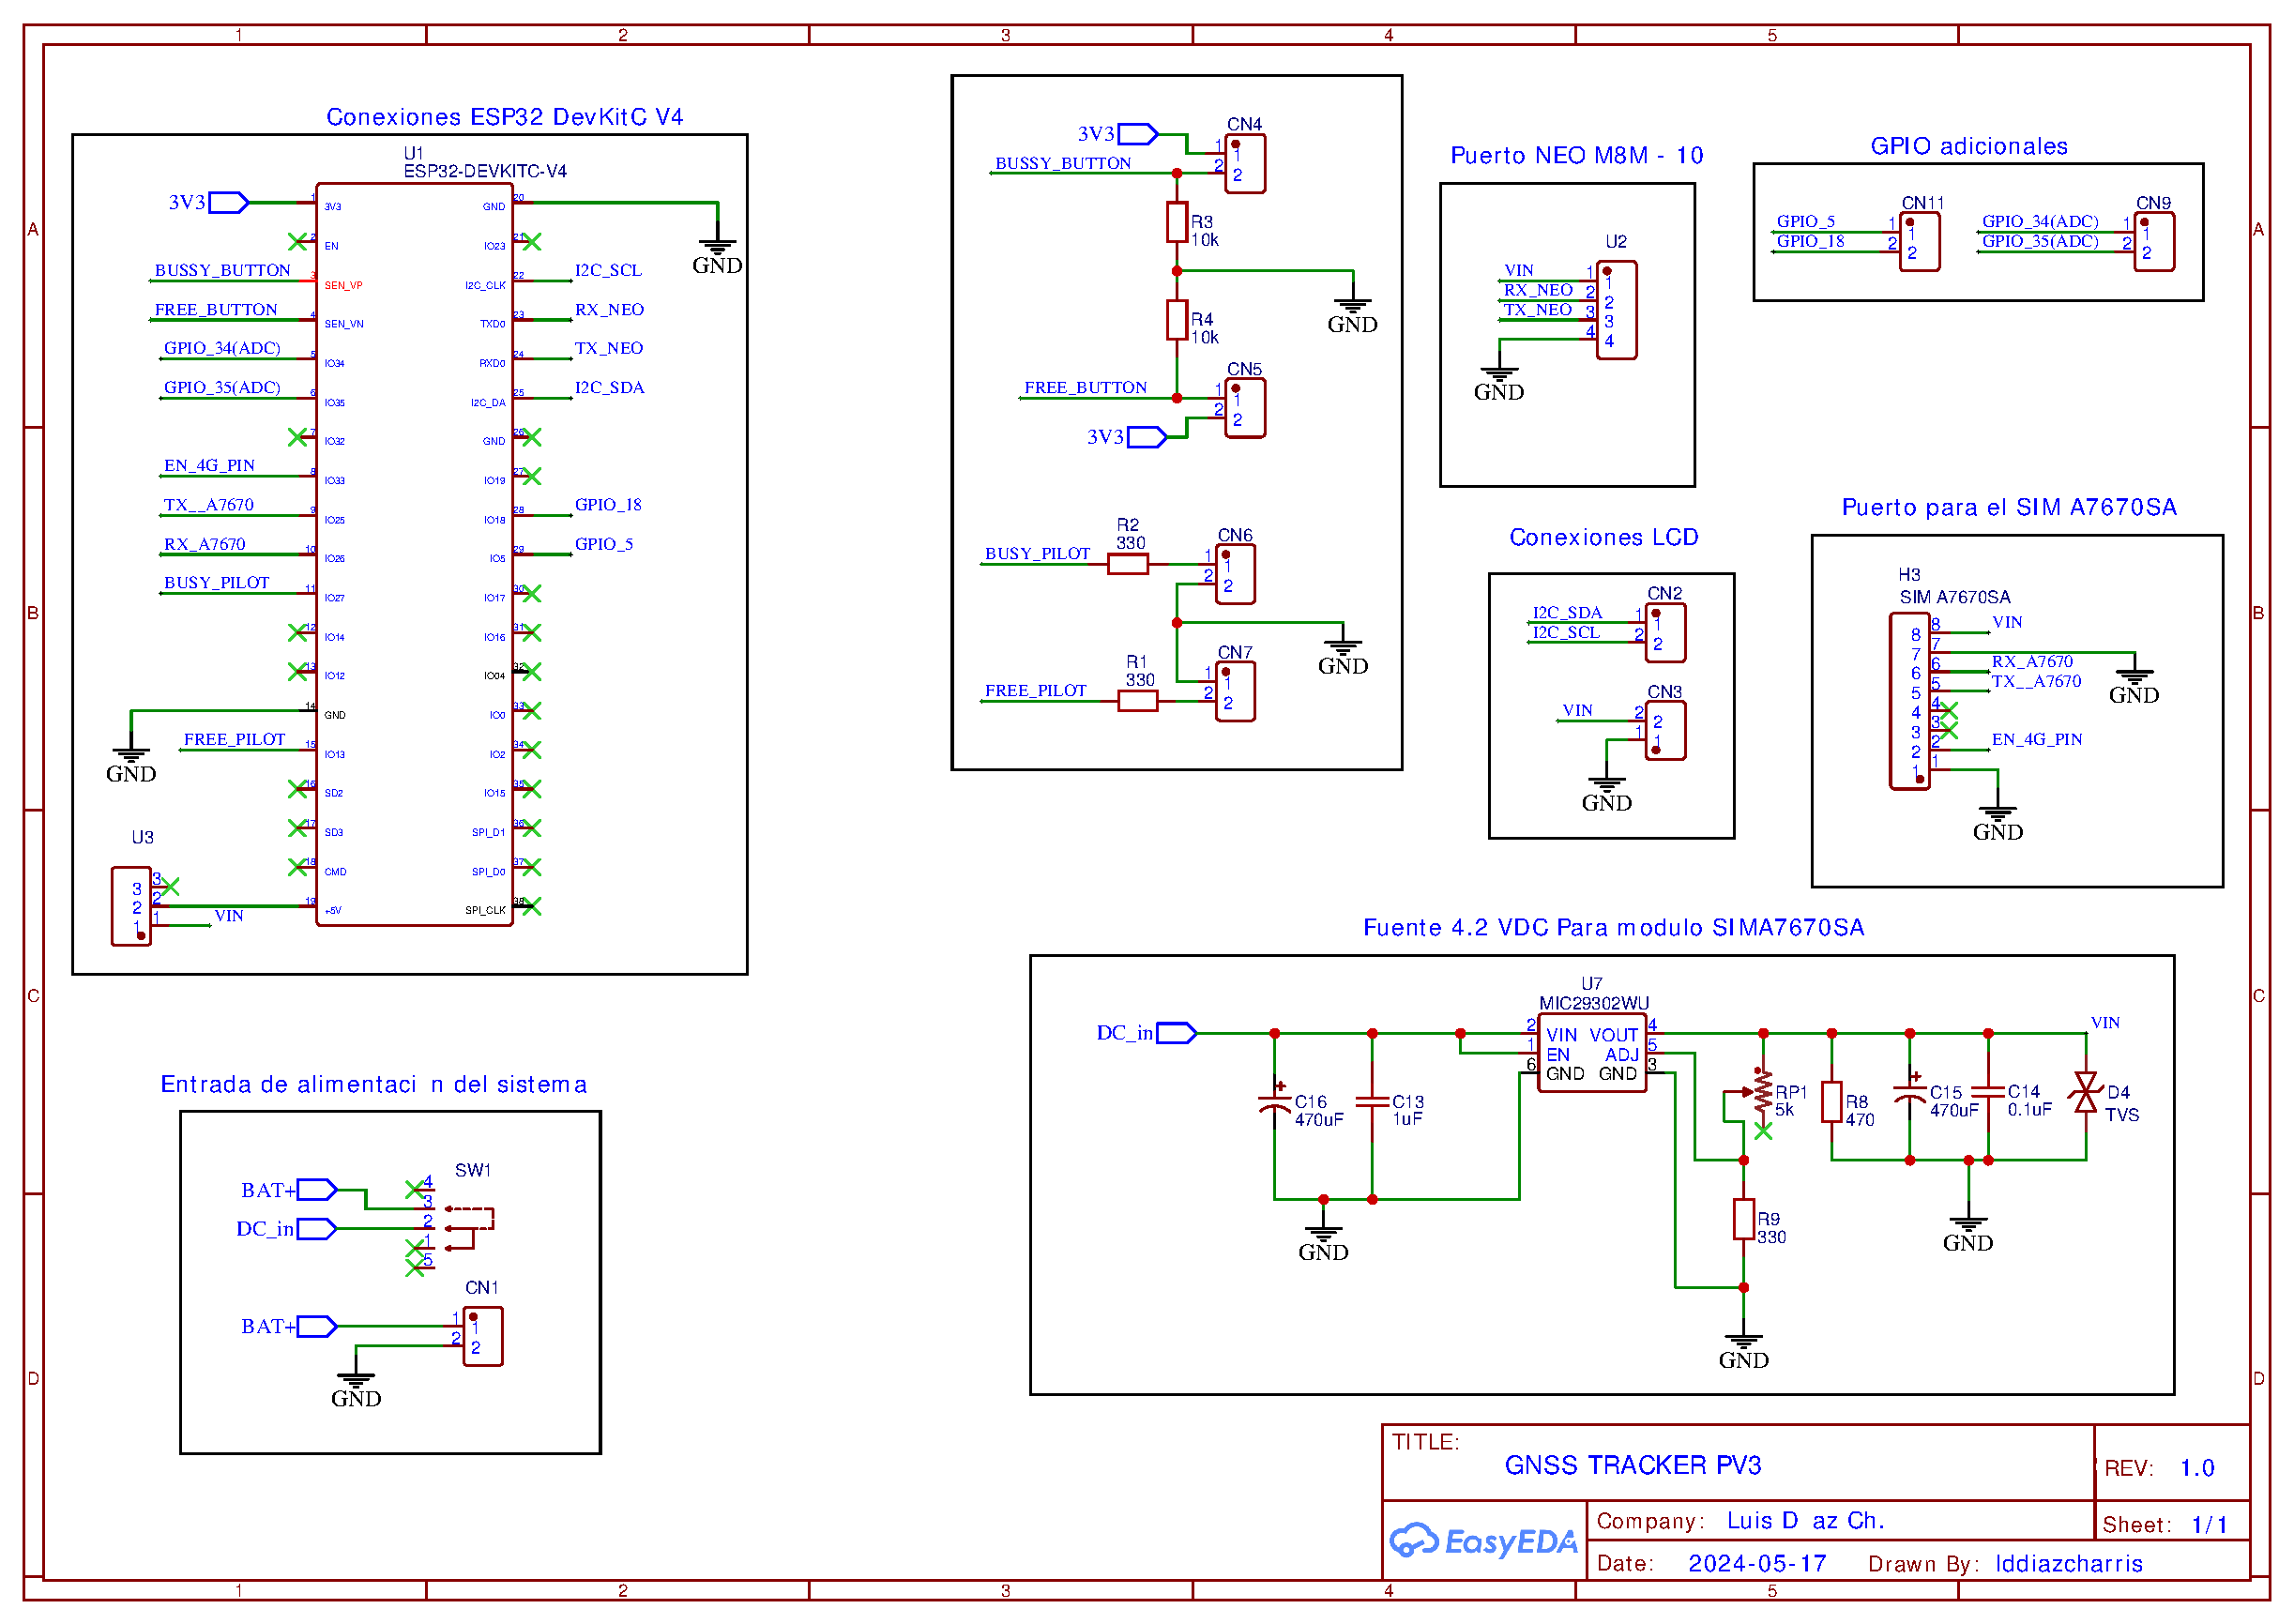
\includegraphics[scale=.3]{./Appendices/Esquematico_placa_base.pdf}


%\begin{figure}[ht]
%	\centering
%	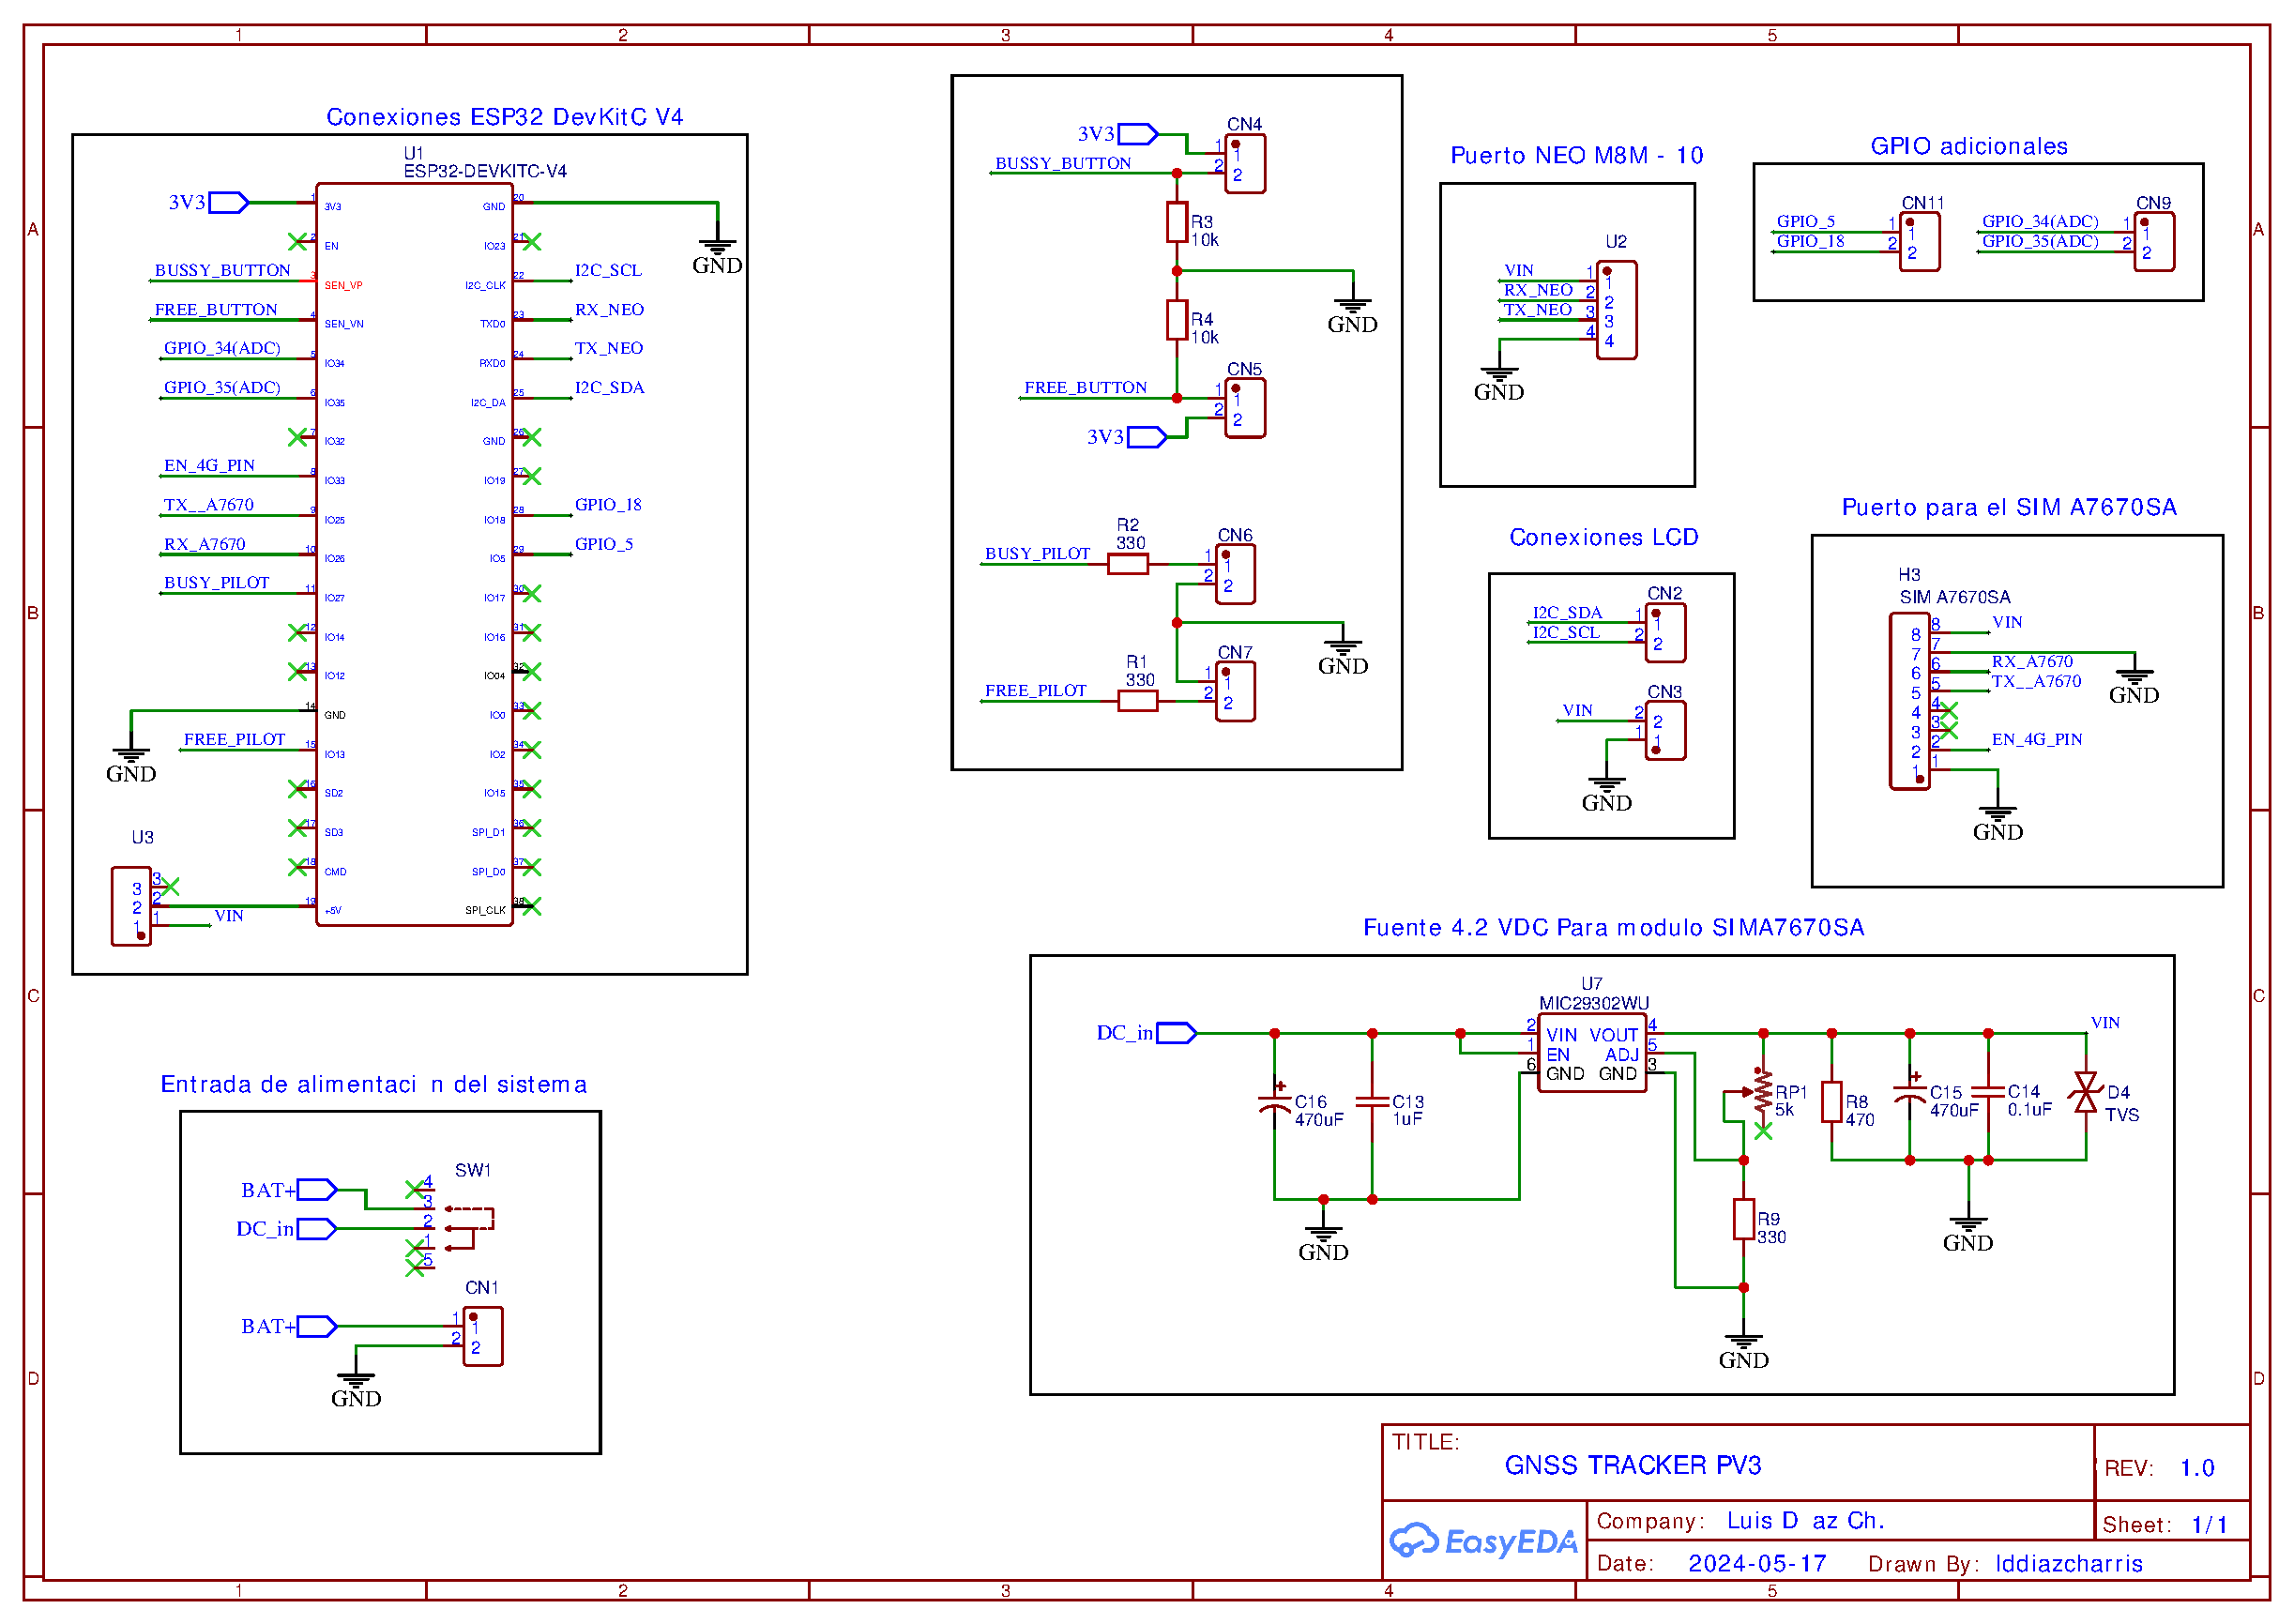
\includegraphics[scale=.5]{./Appendices/Esquematico_placa_base.pdf}
%	\caption{Esquemático de la placa base}
%	\label{fig:placa_base}
%\end{figure}



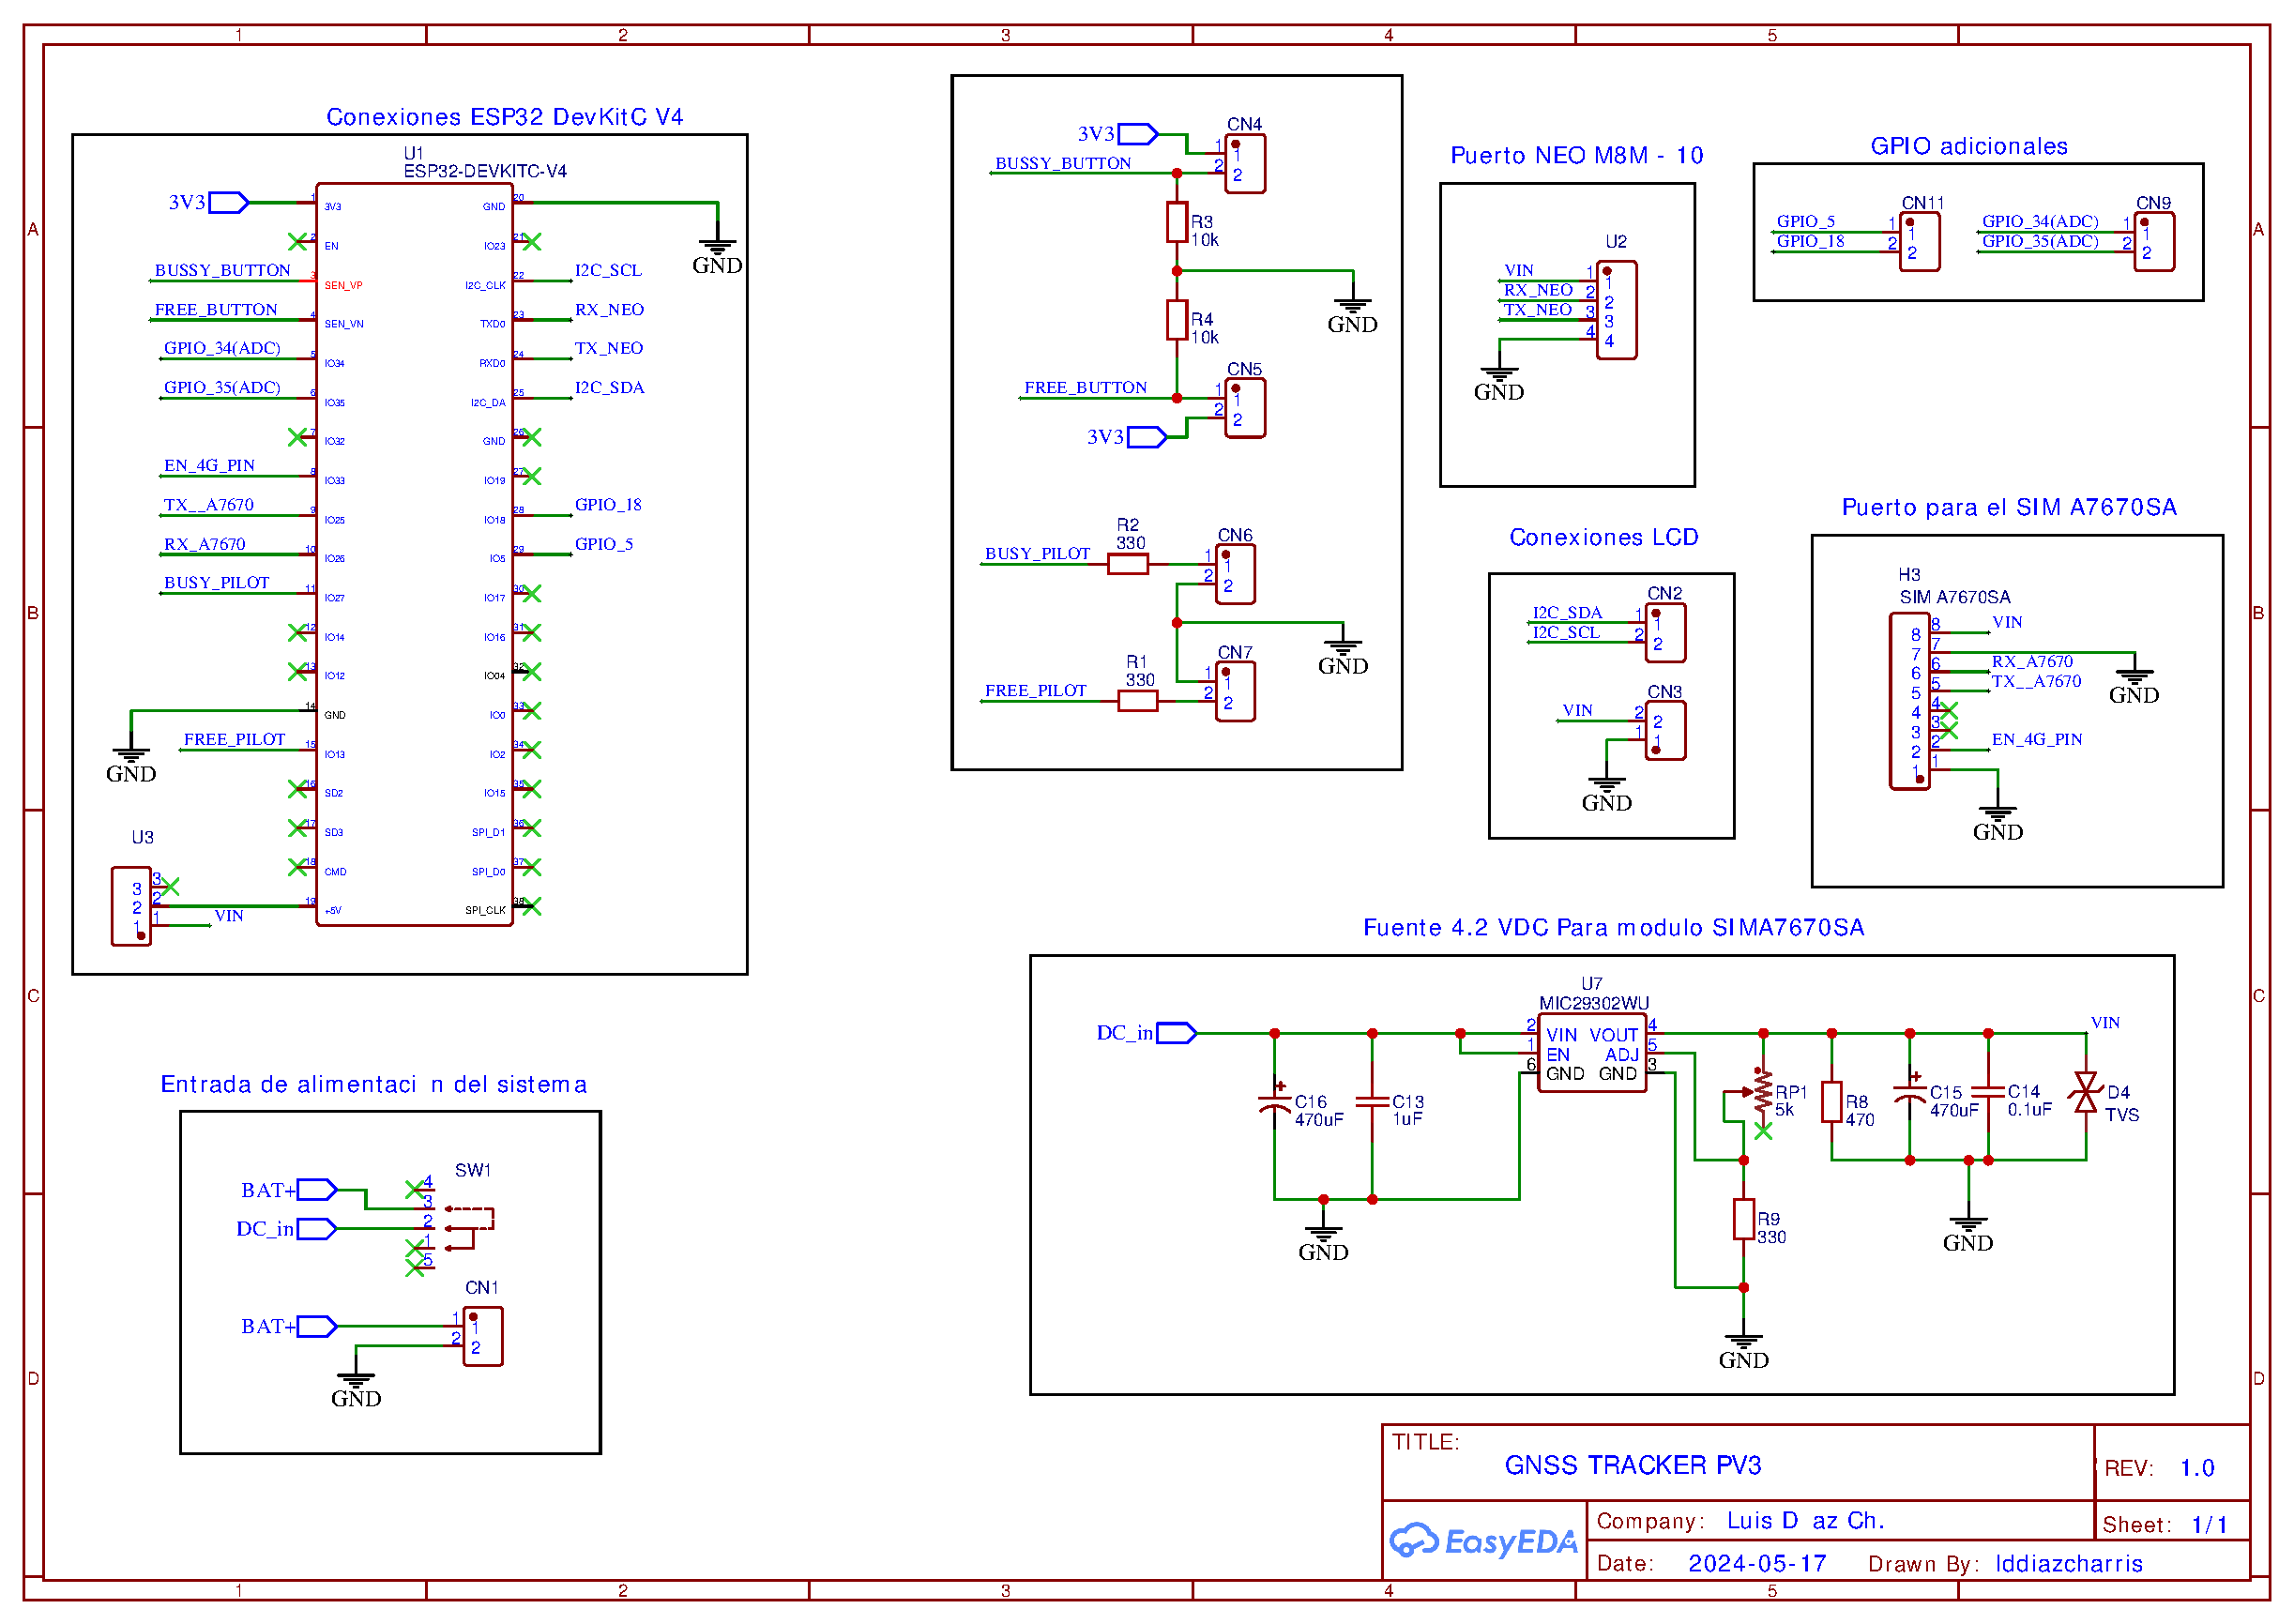
\includepdf[pages=1]{./Appendices/Esquematico_placa_base.pdf}

%\include{Appendices/AppendixB}
%\include{Appendices/AppendixC}

%----------------------------------------------------------------------------------------
%	BIBLIOGRAPHY
%----------------------------------------------------------------------------------------

\Urlmuskip=0mu plus 1mu\relax
\raggedright
\printbibliography[heading=bibintoc]

%----------------------------------------------------------------------------------------

\end{document}  
